\documentclass[chapterprefix=false]{report}
\setlength{\oddsidemargin}{0 in}
\setlength{\evensidemargin}{0 in}
\setlength{\topmargin}{0 in}
\setlength{\textwidth}{5.7 in}
\setlength{\textheight}{8.0 in}
\setlength{\headsep}{0.75 in}
\setlength{\parindent}{0.3 in}
\setlength{\parskip}{0.1 in}
\usepackage{titlesec}

\titleformat{\chapter}{\huge}{\thechapter.}{20pt}{\huge}

\usepackage{epsf}
\usepackage{pseudocode}
\usepackage{amssymb}
\usepackage{mathtools}
\usepackage{amsmath}
\usepackage{algorithm}
\usepackage[noend]{algpseudocode}
\usepackage{textcomp}
\usepackage{tikz}
\usepackage{csquotes}
\usepackage{graphicx}
\usepackage{enumitem}
\usepackage{seqsplit}
\graphicspath{{photos/}}
\usepackage{booktabs}
\usepackage[font=small,labelfont=bf]{caption}
\usepackage{url}
\usepackage{cite}
\usepackage[parfill]{parskip}
\usepackage{setspace}

%\usepackage{titling}
%\renewcommand\maketitlehooka{\null\mbox{}\vfill}
%\renewcommand\maketitlehookd{\vfill\null}

\doublespacing
%\AtBeginEnvironment{tabular}{\singlespacing}
%\AtBeginEnvironment{tabular}{\singlespacing}
\makeatletter
\AtBeginEnvironment{tabular}{%
  \def\baselinestretch{1}\@currsize}%
\makeatother
\usepackage{natbib}
\bibliographystyle{apa}
%\bibliographystyle{unsrtnat}

\usetikzlibrary{arrows}
\tikzset{
    vertex/.style={circle,draw,minimum size=1.5em},
    edge/.style={->,> = latex'}
}

\makeatletter
\def\BState{\State\hskip-\ALG@thistlm}
\makeatother

\DeclarePairedDelimiter\ceil{\lceil}{\rceil}
\DeclarePairedDelimiter\floor{\lfloor}{\rfloor}

% \usepackage{times}
% \usepackage{mathptm}

\def\O{\mathop{\smash{O}}\nolimits}
\def\o{\mathop{\smash{o}}\nolimits}
\newcommand{\e}{{\rm e}}
\newcommand{\R}{{\bf R}}
\newcommand{\Z}{{\bf Z}}
\newcommand{\h}{1.2}


\DeclareMathOperator*{\argmin}{arg\,min}
\DeclareMathOperator*{\argmax}{arg\,max}
 
\begin{document}
\linespread{2}

\section*{Acknowledgements}

After coming across Michael Sipko's ``Machine Learning for the Prediction of Professional Tennis Matches,'' I realized that I could write my senior thesis on the sport I am most passionate about. While I was abroad this past summer, much of this project's implementation took place in caf\'{e}s around Tokyo, Japan. Thank you to my advisor, Kevin Rader, for his enthusiasm and support. Thank you to my parents, for pushing me to make the most out of my academic opportunities at college. Finally, thank you to my former coaches Joaqu\'{i}n, Stewart, and Paul for their lessons and wisdom over the years. My lifelong obsession with tennis persists through this project.

%played in tournaments and high school
 
\tableofcontents{}
 
\chapter{Introduction}
 
\section{In-game Sports Analytics}

$\newline$
``The win probability graphic/discussion on ESPN is literally taking a sword and sticking it through the chest of any fun left in baseball''
\\[5pt]
\centerline{{ --- Kenny Ducey (@KennyDucey) April 2, 2017}}

$\newline$
``ESPN showing win probability is extremely good. Next up, run expectancy!''
\\[5pt]
\centerline{{\rm --- Neil Weinberg (@NeilWeinberg44) April 4, 2017}}

``Thank the Lord we have the ESPN Win Probability stat to tell us the team that's ahead has a good chance to win.''
\\[5pt]
\centerline{{\rm --- Christian Schneider (@Schneider\_CM) April 17, 2017}}

In recent years, win probability has become increasingly prevalent in sports broadcasting. Brian Burke, an NFL commentator, has posted live win-probability graphs of NFL playoff games on his website for the past few years \citep{WPexp}. Earlier this year, ESPN began to post win probabilities atop the score box in televised Major League Baseball games \citep{ESPNwp}. Despite mixed reactions from fans, as shown above, these developments represent a transition in sports broadcasting's modern narrative. 

%..Make an argument for the value of in-match forecasting, despite angry reactions..

A win probability from any scoreline communicates how much a team or player is favored to win. While one can produce this from any model of choice, those in sports analytics strive to produce the most well-informed estimate available.  With the recent proliferation of online betting, in-match win probability dictates an entire market of its own. Betfair's platform  matched over 40 million euro during the 2011 French Open Final \citep{Huang2011}; other high-profile matches often draw comparable volume over betting exchanges. While the majority of tennis prediction papers concern pre-match prediction, around 80$\%$ of online betting occurs while matches are in progress \citep{Sipko2015}. At the very least, in-match win probability concerns all participants in this betting market.

%While one can produce this from any model of choice, sports analytics strives to produce the most well-informed estimate available. 
%While tennis has yet to broadcast win probabilities, 

%demonstrates an individual model’s most informed guess at how likely a player is to win the match

%Drawing upon past research and exploring new methods, this paper searches for the most effective approach to in-match forecasting.

\section{History of Tennis Forecasting}
%Plenty of research on tennis match prediction exists over the past twenty years. 

Statistical prediction models have been applied to tennis matches for over twenty years. Klaassen and Magnus tested the assumption that points in a tennis match are independent and identically distributed, or i.i.d. \citep{KlaassenandMagnus2001}. While the assumption is false, they concluded that deviations are small enough that constant probabilities provide a reasonable approximation. Under this assumption, they construct a hierarchical Markov model in conjunction with tennis' scoring system. From this model, they offer an analytical equation for match-win probability from any score, given each individual player's probability of winning a point on serve \citep{Klaassen2003}.  Barnett and Clarke then offer a method of estimating each player's serve probability from historical data \citep{BarnettandClarke2005}. Years later, Bevc proposed updating each of these serve probabilities with a beta distribution between each point and computing the corresponding win probability with the above model \citep{Bevc2015}. Recently, Kovalchik assessed performance of 11 different pre-match prediction models on 2014 ATP tour-level matches. While the market-based Bookmaker Consensus Model performed best overall, Elo ratings proved most effective among methods that rely on historical data \citep{Kovalchik2016}.

Over the past several years, Jeff Sackmann has released the largest publicly available library of tennis datasets via github. This collection contains match summaries of every ATP and WTA match in the Open Era, point-by-point summaries of nearly 100,000 tour-level and satellite matches, and a crowd-sourced match-charting project spanning over 3,000 matches, where volunteers record each shot's type and direction over an entire match. While FiveThirtyEight and Kovalchik have used Jeff Sackmann’s match data to generate Elo ratings, none of the aforementioned papers have tested models with his point-by-point dataset.

As past papers have spanned several decades, datasets and model evaluation are not consistent. Klaassen and Magnus' original point-based model and Bevc's beta experiments both apply methods to around 500 Wimbledon matches from 1991-94. Barnett explores point-based models in great depth, yet primarily applies them to a single marathon match between Andy Roddick and Younes El Aynaoui from the 2002 Australian Open \citep{Barnett2006}. Except for Bevc, none of these papers assess in-game match prediction with metrics such as accuracy or cross-entropy. While Bevc does record accuracy of results over 500 Wimbledon matches, he only reports accuracy of predictions in the third set and onwards, a subset of the entire dataset. In other words, no one has taken all in-game prediction models and tested them at a large scale. For this reason, I will test all relevant in-match prediction methods on thousands of matches within the past seven years.

%However, Jeff Sackmann has recently released the largest publicly available tennis dataset via github. This collection contains match summaries of every ATP and WTA match in the Open Era, point-by-point summaries of nearly 100,000 matches—both tour-level and satellite--and a crowd-sourced match-charting project spanning 2800 matches, where volunteers record each shot’s type and direction in every point. While 538 and Kovalchik use Jeff Sackmann’s match data to refine their own Elo system for pre-match prediction, no papers on in-match prediction have used his point-by-point dataset. With over 10,000 ATP and WTA tour-level matches from 2010-2017, I compare existing approaches side-by-side and explore new methods to in-match prediction.  Just as Kovalchik does with pre-match prediction models, I attempt to find the GOAT (greatest of all-time) of in-match prediction models.

This paper combines Elo ratings, a wealth of data, and current technology to provide a similar survey of which in-match prediction methods perform the best. We build upon past research by testing variations of previous state-of-the-art methods, and applying new concepts to these datasets, from Random Forest models used in football to elo-induced serving percentages.
 
\section{Match/Point-by-Point Datasets}
 
This project uses two different types of datasets: one with match summary statistics and one with point-by-point information. Both are publicly available on github, courtesy of Jeff Sackmann (\url{https://github.com/JeffSackmann}). We use the matches dataset under ``\texttt{tennis\_atp}'' to test pre-match prediction methods. This dataset covers over 150,000 tour-level matches, dating back to 1968. Relevant features include:

\begin{itemize}
  \item match info (date, tournament, player names)
  \item match statistics (serve/return match statistics for each player)
\end{itemize}


The data in ``\texttt{tennis\_pointbypoint}'' offers more granular detail about a single match's point progression. Each match contains a string listing the order in which players won points and switched serve. While \url{atpworldtour.com} does not publicly list point-by-point summaries, Jeff Sackmann has made this information available from a betting website. Unlike the match dataset, this dataset covers around 12,000 tour-level matches dating back to 2010. Relevant features include:

\begin{itemize}
  \item match info (date, tournament, player names)
  \item point-by-point (a string detailing the sequence in which points were won)
\end{itemize}

\section{Implementation}

With the above datasets serving as a basis for this project, thorough re-formatting of the data was required in order to connect point-by-point strings to their corresponding observations in the match dataset. As both datasets included player names, year, and score, we connected matches across datasets with a hashing scheme.\footnote{eg. hash(matchX) = ``Roger Federer Tomas Berdych 2012 3-6 7-5 7-5''} Due to observed inconsistencies, we standardized player names between match and point-by-point datasets in order to maximize the number of available matches with point-by-point summaries.$\footnote{eg. ``Stan Wawrinka'' $\rightarrow$ ``Stanislas Wawrinka'', ``Federico Del Bonis'' $\rightarrow$ ``Federico Delbonis''}$ While a portion of the point-by-point summaries are from satellite events, akin to the minor leagues of tennis, we were able to match around 10,600/12,000 point-by-point strings to their respective tour-level matches. Then, we could associate information generated from the match dataset's entirety (Elo ratings, year-long adjusted serve stats, etc) with corresponding point-by-point strings.

To view this process in more depth or access any of the resulting datasets, visit \url{https://github.com/jgollub1/tennis_match_prediction}. Implementations of each method in this project\footnote{All methods covered in this project required feature construction across the two datasets.}, and instructions on how to generate all relevant statistics, are also provided.

\chapter{Scoring}
Tennis' scoring system consists of three levels: sets, games, and points. Consider a tennis match between two entities, $p_i$ and $p_j$. We can represent any score as $(s_i,s_j,g_i,g_j,{x}_i,{x}_j)$ where $p_i$ is serving and $s_k,g_k,x_k$ represent $p_k$'s score in sets, games, and points, respectively.$\footnote{While tennis officially  refers to a game's first three points as 15,30,40 we will call them 1,2,3 for simplicity's sake.}$ The players alternate serve each game and continue until someone clinches the match by winning two sets (best-of-three) or three sets (best-of-five).$\footnote{The best-of-five format is typically reserved for men's grand slam and Davis Cup events.}$

The majority of in-play tennis models utilize a graphical structure that embodies the levels within tennis' scoring system. Madurska referred to this as a hierarchical Markov Model \citep{madurska2012set}. Barnett formally defines this representation for tennis scores \citep{BarnettandClarke2002}. With $p_i$ and $p_j$ winning points on serve with probabilities $f_{ij},f_{ji}$, each in-match scoreline $(s_i,s_j,g_i,g_j,{x}_i,{x}_j)$ progresses to one of its two neighbors $(s_i,s_j,g_i,g_j,{x}_i+1,{x}_j)$ and $(s_i,s_j,g_i,g_j,{x}_i,{x}_j+1)$ with transition probabilities dependent on the current server. Assuming all points in a match are i.i.d. between servers, we can then use the below model to recursively determine win probability. Consider the scoreboard below, with Rafael Nadal serving to Juan Martin Del Potro 7-6 3-6 6-6 2-1, in the 2011 Wimbledon 4th round. Representing the score from the server's point of view, we find:

%$P_m(s_i,s_j,g_i,g_j,{x}_i,{x}_j)$ = probability that $p_i$ wins the match when serving from this scoreline$P_m(s_i,s_j,g_i,g_j,{x}_i,{x}_j) = f_{ij}*P_m(s_i,s_j,g_i,g_j,{x}_i+1,{x}_j) + (1-f_{ij}) P_m(s_i,s_j,g_i,g_j,{x}_i,{x}_j+1)$

\begin{center}

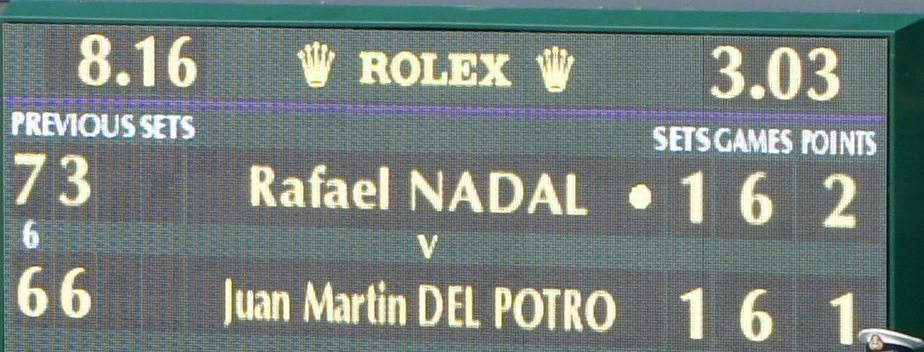
\includegraphics[scale=.3]{scoreboard}
\captionof{figure}{Nadal serving to Del Potro in a third set tiebreakerc}

$P_m(1,1,6,6,2,1)$ = P($p_i$ wins the match, serving from this scoreline)

$P_m(1,1,6,6,2,1) = f_{ij}*P_m(1,1,6,6,3,1) + (1-f_{ij}) P_m(1,1,6,6,2,2)$


\end{center}
In the following sections, we specify boundary values to each level of our hierarchical model. 

%With these specifications, we can analytically compute win probability at any point in the match.


\section{Modeling games}

Within a game, either $p_i$ or $p_j$ serves every point. Every game starts at (0,0) and to win a game, a player must win four or more points by a margin of at least two. Consequently, all games with valid scores $(x_i,x_j)$ where $x_i+x_j$ \textgreater $6,$ $|x_i-x_j| \leq 1$ are reduced to (3,3), (3,2), or (2,3). Furthermore, the win probability at (3,3) can be calculated directly. From (3,3), the server wins the next two points with probability $(f_{ij})^2$, the returner wins the next two points with probability $(1-f_{ij})^2$, or both players split the two points and return to (3,3) with probability $2f_{ij}(1-f_{ij})$. Relating the game's remainder to a geometric sequence, we find $P_g(3,3) = \dfrac{(f_{ij})^2}{(f_{ij})^2+(1-f_{ij})^2}$. As the probability of winning each point remains constant for both players, this graph assumes that points within a game are independent. In the following levels, we assume that games within a set and sets within a match are independent.

Possible sequences of point scores in a game:

a - $p_i$ wins the following point

b - $p_j$ wins the following point

\begin{tikzpicture} [scale=1]
\tikzset{VertexStyle/.style = {shape = circle,inner sep=0x}}
\node[vertex] (1) at (0,0) {$0,0$};
\node[vertex] (2) at (2,.8) {$1,0$};
\node[vertex] (3) at (2,-.8) {$0,1$};
\node[vertex] (4) at (4,0) {$1,1$};
\node[vertex] (7) at (4,1.6) {$2,0$};
\node[vertex] (8) at (4,-1.6) {$0,2$};
\node[vertex] (5) at (6,.8) {$2,1$};
\node[vertex] (6) at (6,-.8) {$1,2$};
\node[vertex] (9) at (6,2.4) {$3,0$};
\node[vertex] (10) at (6,-2.4) {$0,3$};
\node[vertex] (11) at (8,1.6) {$3,1$};
\node[vertex] (12) at (8,-1.6) {$1,3$};
\node[vertex] (13) at (8,0) {$2,2$};

\node[vertex] (14) at (12,3.2) {$G_1$};
\node[vertex] (15) at (12,-3.2) {$G_1^{c}$};
\node[vertex] (16) at (10,.8) {$3,2$};
\node[vertex] (17) at (10,-.8) {$2,3$};
\node[vertex] (18) at (12,0) {$3,3$};

\draw[edge] (1) -- (2) node[midway, above] {$a$};
\draw[edge] (1) -- (3) node[midway, above] {$b$};
\draw[edge] (2) -- (4) node[midway, above] {$b$};
\draw[edge] (3) -- (4) node[midway, above] {$a$};
\draw[edge] (2) -- (7) node[midway, above] {$a$};
\draw[edge] (3) -- (8) node[midway, above] {$b$};
\draw[edge] (4) -- (5) node[midway, above] {$a$};
\draw[edge] (4) -- (6) node[midway, above] {$b$};
\draw[edge] (7) -- (9) node[midway, above] {$a$};
\draw[edge] (7) -- (5) node[midway, above] {$b$};
\draw[edge] (8) -- (6) node[midway, above] {$a$};
\draw[edge] (8) -- (10) node[midway, above] {$b$};
\draw[edge] (9) -- (11) node[midway, above] {$b$};
\draw[edge] (10) -- (12) node[midway, above] {$a$};
\draw[edge] (5) -- (11) node[midway, above] {$a$};
\draw[edge] (6) -- (12) node[midway, above] {$b$};
\draw[edge] (5) -- (13) node[midway, above] {$b$};
\draw[edge] (6) -- (13) node[midway, above] {$a$};
\draw[edge] (13) -- (16) node[midway, above] {$a$};
\draw[edge] (13) -- (17) node[midway, above] {$b$};
\draw[edge] (11) -- (16) node[midway, above] {$b$};
\draw[edge] (12) -- (17) node[midway, above] {$a$};
\draw[edge] (16) -- (18) node[midway, above] {$b$};
\draw[edge] (17) -- (18) node[midway, above] {$a$};
\draw[edge] (9) -- (14) node[midway, above] {$a$};
\draw[edge] (11) -- (14) node[midway, above] {$a$};
\draw[edge] (16) -- (14) node[midway, above] {$a$};
\draw[edge] (10) -- (15) node[midway, above] {$b$};
\draw[edge] (12) -- (15) node[midway, above] {$b$};
\draw[edge] (17) -- (15) node[midway, above] {$b$};
\draw[->, xshift=11.3cm, yshift=1cm] (18) to [bend right=50] (16) node[ sloped,midway,above] {$a$};
\draw[->, xshift=11.3cm, yshift=-1cm] (18) to [bend left=50] (17) node[ sloped,midway,above] {$b$};

\end{tikzpicture}

Boundary values:

\begin{equation}
    P_g(x_i,x_j) 
    \begin{cases}
      1, & \text{if}\ x_1=4,x_2 \leq 2 \\
      0, & \text{if}\ x_2=4,x_1 \leq 2 \\
      \cfrac{(f_{ij})^2}{(f_{ij})^2+(1-f_{ij})^2}, & \text{if}\ x_1=x_2=3 \\
      f_{ij}*P_g(s_i,s_j,g_i,g_j,{x}_i+1,{x}_j) + (1-f_{ij}) P_g(s_i,s_j,g_i,g_j,{x}_i,{x}_j+1), & \text{otherwise}\ \\
      
    \end{cases}
  \end{equation}

With the above specifications, we can efficiently compute $p_i$'s win probability from any score $P_g(x_i,x_j)$.

\section{Modeling sets}

Within a set, $p_i$ or $p_j$ alternate serve every game. Every set starts at (0,0). To win a set, a player must win six or more games by a margin of at least two. If the set score $(6,6)$ is reached, a special tiebreaker game is played to determine the outcome of the match.

Possible sequences of point scores in a game:

$a$ - player 1 wins the following game

$b$ - player 2 wins the following game

$a'$ - player 1 wins the tiebreaker game

$b'$ - player 2 wins the tiebreaker game

\begin{tikzpicture} [scale=.7]
\tikzset{VertexStyle/.style = {shape = circle,inner sep=0x}}
\node[vertex] (1) at (0,0) {$0,0$};
\node[vertex] (2) at (2,\h) {$1,0$};
\node[vertex] (3) at (2,-\h) {$0,1$};
\node[vertex] (4) at (4,2*\h) {$2,0$};
\node[vertex] (5) at (4,0) {$1,1$};
\node[vertex] (6) at (4,-2*\h) {$0,2$};
\node[vertex] (7) at (6,3*\h) {$3,0$};
\node[vertex] (8) at (6,\h) {$2,1$};
\node[vertex] (9) at (6,-\h) {$1,2$};
\node[vertex] (10) at (6,-3*\h) {$0,3$};
\node[vertex] (11) at (8,4*\h) {$4,0$};
\node[vertex] (12) at (8,2*\h) {$3,1$};
\node[vertex] (13) at (8,0) {$2,2$};
\node[vertex] (14) at (8,-2*\h) {$1,3$};
\node[vertex] (15) at (8,-4*\h) {$0,4$};
\node[vertex] (16) at (10,5*\h) {$5,0$};
\node[vertex] (17) at (10,3*\h) {$4,1$};
\node[vertex] (18) at (10,\h) {$3,2$};
\node[vertex] (19) at (10,-\h) {$2,3$};
\node[vertex] (20) at (10,-3*\h) {$1,4$};
\node[vertex] (21) at (10,-5*\h) {$0,5$};
\node[vertex] (22) at (18,6*\h) {$S_1$};
\node[vertex] (23) at (12,4*\h) {$5,1$};
\node[vertex] (24) at (12,2*\h) {$4,2$};
\node[vertex] (25) at (12,0) {$3,3$};
\node[vertex] (26) at (12,-2*\h) {$2,4$};
\node[vertex] (27) at (12,-4*\h) {$1,5$};
\node[vertex] (28) at (18,-6*\h) {$S_1^c$};
\node[vertex] (29) at (14,3*\h) {$5,2$};
\node[vertex] (30) at (14,\h) {$4,3$};
\node[vertex] (31) at (14,-\h) {$3,4$};
\node[vertex] (32) at (14,-3*\h) {$2,5$};
\node[vertex] (33) at (16,2*\h) {$5,3$};
\node[vertex] (34) at (16,0) {$4,4$};
\node[vertex] (35) at (16,-2*\h) {$3,5$};
\node[vertex] (36) at (18,\h) {$5,4$};
\node[vertex] (37) at (18,-\h) {$4,5$};
\node[vertex] (38) at (20,0) {$5,5$};
\node[vertex] (39) at (22,\h) {$6,5$};
\node[vertex] (40) at (22,-\h) {$5,6$};
\node[vertex] (41) at (24,0) {$6,6$};



\draw[edge] (1) -- (2) node[midway, above] {$a$};
\draw[edge] (1) -- (3) node[midway, above] {$b$};
\draw[edge] (2) -- (4) node[midway, above] {$b$};
\draw[edge] (2) -- (5) node[midway, above] {$a$};
\draw[edge] (3) -- (5) node[midway, above] {$a$};
\draw[edge] (3) -- (6) node[midway, above] {$b$};
\draw[edge] (4) -- (7) node[midway, above] {$a$};
\draw[edge] (4) -- (8) node[midway, above] {$b$};
\draw[edge] (5) -- (8) node[midway, above] {$a$};
\draw[edge] (5) -- (9) node[midway, above] {$b$};
\draw[edge] (6) -- (9) node[midway, above] {$a$};
\draw[edge] (6) -- (10) node[midway, above] {$b$};
\draw[edge] (7) -- (11) node[midway, above] {$a$};
\draw[edge] (7) -- (12) node[midway, above] {$b$};
\draw[edge] (8) -- (12) node[midway, above] {$a$};
\draw[edge] (8) -- (13) node[midway, above] {$b$};
\draw[edge] (9) -- (13) node[midway, above] {$a$};
\draw[edge] (9) -- (14) node[midway, above] {$b$};
\draw[edge] (10) -- (14) node[midway, above] {$a$};
\draw[edge] (10) -- (15) node[midway, above] {$b$};
\draw[edge] (11) -- (16) node[midway, above] {$a$};
\draw[edge] (11) -- (17) node[midway, above] {$b$};
\draw[edge] (12) -- (17) node[midway, above] {$a$};
\draw[edge] (12) -- (18) node[midway, above] {$b$};
\draw[edge] (13) -- (18) node[midway, above] {$a$};
\draw[edge] (13) -- (19) node[midway, above] {$b$};
\draw[edge] (14) -- (19) node[midway, above] {$a$};
\draw[edge] (14) -- (20) node[midway, above] {$b$};
\draw[edge] (15) -- (20) node[midway, above] {$a$};
\draw[edge] (15) -- (21) node[midway, above] {$b$};
\draw[edge] (16) -- (22) node[midway, above] {$a$};
\draw[edge] (16) -- (23) node[midway, above] {$b$};
\draw[edge] (17) -- (23) node[midway, above] {$a$};
\draw[edge] (17) -- (24) node[midway, above] {$b$};
\draw[edge] (18) -- (24) node[midway, above] {$a$};
\draw[edge] (18) -- (25) node[midway, above] {$b$};
\draw[edge] (19) -- (25) node[midway, above] {$a$};
\draw[edge] (19) -- (26) node[midway, above] {$b$};
\draw[edge] (20) -- (26) node[midway, above] {$a$};
\draw[edge] (20) -- (27) node[midway, above] {$b$};
\draw[edge] (21) -- (27) node[midway, above] {$a$};
\draw[edge] (21) -- (28) node[midway, above] {$b$};
\draw[edge] (23) -- (22) node[midway, above] {$a$};
\draw[edge] (23) -- (29) node[midway, above] {$b$};
\draw[edge] (24) -- (29) node[midway, above] {$a$};
\draw[edge] (24) -- (30) node[midway, above] {$b$};
\draw[edge] (25) -- (30) node[midway, above] {$a$};
\draw[edge] (25) -- (31) node[midway, above] {$b$};
\draw[edge] (26) -- (31) node[midway, above] {$a$};
\draw[edge] (26) -- (32) node[midway, above] {$b$};
\draw[edge] (27) -- (32) node[midway, above] {$a$};
\draw[edge] (27) -- (28) node[midway, above] {$b$};
\draw[edge] (29) -- (22) node[midway, above] {$a$};
\draw[edge] (29) -- (33) node[midway, above] {$b$};
\draw[edge] (30) -- (33) node[midway, above] {$a$};
\draw[edge] (30) -- (34) node[midway, above] {$b$};
\draw[edge] (31) -- (34) node[midway, above] {$a$};
\draw[edge] (31) -- (35) node[midway, above] {$b$};
\draw[edge] (32) -- (35) node[midway, above] {$a$};
\draw[edge] (32) -- (28) node[midway, above] {$b$};
\draw[edge] (33) -- (22) node[midway, above] {$a$};
\draw[edge] (33) -- (36) node[midway, above] {$b$};
\draw[edge] (34) -- (36) node[midway, above] {$a$};
\draw[edge] (34) -- (37) node[midway, above] {$b$};
\draw[edge] (35) -- (37) node[midway, above] {$a$};
\draw[edge] (35) -- (28) node[midway, above] {$b$};
\draw[edge] (36) -- (22) node[midway, left] {$a$};
\draw[edge] (36) -- (38) node[midway, above] {$b$};
\draw[edge] (37) -- (38) node[midway, above] {$a$};
\draw[edge] (37) -- (28) node[midway, right] {$b$};
\draw[edge] (38) -- (39) node[midway, above] {$a$};
\draw[edge] (38) -- (40) node[midway, above] {$b$};
\draw[edge] (39) -- (22) node[midway, above] {$a$};
\draw[edge] (39) -- (41) node[midway, above] {$b$};
\draw[edge] (40) -- (41) node[midway, above] {$a$};
\draw[edge] (40) -- (28) node[midway, above] {$b$};

\draw[->, xshift=20cm,yshift=6.35cm] (41) to [bend right=30] (22) node[sloped,midway,above,scale=1.4] {$a'$};
\draw[->, xshift=20cm,yshift=-6.35cm] (41) to [bend left=30] (28) node[sloped,midway,above,scale=1.4] {$b'$};


\end{tikzpicture}

Boundary values:
\begin{equation}
    P_s(g_1,g_2) 
    \begin{cases}
      1, & \text{if}\ g_1 \geq 6,g_1-g_2 \geq 2 \\
      0, & \text{if}\ g_2 \geq 6,g_2-g_1 \geq 2 \\
      P_{tb}(s_1,s_2), & \text{if}\ g_1=g_2=6 \\
      P_g(0,0)(1-P_s(g_2,g_1+1))+(1-P_g(0,0))(1-P_s(g_2+1,g_1)), & \text{otherwise}\ \\
    \end{cases}
  \end{equation}

\section{Modeling a tiebreak game}

Within a tiebreak game, one player serves the first point and players alternate serve every two points from then on. The game starts at (0,0) and a player must win seven points by a margin of two or more to win.

Boundary values:
\begin{equation}
    P_t(p_1,p_2) 
    \begin{cases}
      1, & \text{if}\ p_1 \geq 7,p_1-p_2 \geq 2 \\
      0, & \text{if}\ p_2 \geq 7,p_2-p_1 \geq 2 \\
      f_{ij}P_t(g_1+1,g_2)+(1-f_{ij})P_t(g_1,g_2+1), & \text{if}\ (p_1+p_2) \mod 2 = 1 \\
f_{ij}(1-P_t(g_2,g_1+1))+(1-f_{ij})(1-P_t(g_2+1,g_1)), & \text{if}\ (p_1+p_2) \mod 2 = 0 \\
    \end{cases}
  \end{equation}

\section{Modeling a best-of-three match}

In a best-of-three match, the first player to win two sets claims the match. This project primarily applies models to best-of-three matches. In a best-of-five match, the graph would have boundary values at $s_1 \geq 3, s_2 \geq 3$ at 3, since a player must win three sets to finish the match. 

$a$ - player 1 wins the following set

$b$ - player 2 wins the following set

\begin{tikzpicture} [scale=1]
\node[vertex] (1) at (0,0) {$0,0$};
\node[vertex] (2) at (2,1) {$1,0$};
\node[vertex] (3) at (2,-1) {$0,1$};
\node[vertex] (4) at (4,0) {$1,1$};
\node[vertex] (5) at (6,1) {$W_1$};
\node[vertex] (6) at (6,-1) {$W_1^{c}$};

\draw[edge] (1) -- (2) node[midway, above] {$a$};
\draw[edge] (1) -- (3) node[midway, above] {$b$};
\draw[edge] (2) -- (4) node[midway, above] {$b$};
\draw[edge] (3) -- (4) node[midway, above] {$a$};
\draw[edge] (2) -- (5) node[midway, above] {$a$};
\draw[edge] (3) -- (6) node[midway, above] {$b$};
\draw[edge] (4) -- (5) node[midway, above] {$a$};
\draw[edge] (4) -- (6) node[midway, above] {$b$};

\end{tikzpicture}

Boundary values:
\begin{equation}
    P_m(s_1,s_2) 
    \begin{cases}
      1, & \text{if}\ s_1 \geq 2 \\
      0, & \text{if}\ s_2 \geq 2 \\
      P_s(0,0)(P_m(s_1+1,s_2))+(1-P_s(0,0))(P_m(s_1,s_2+1)), & \text{otherwise}\ \\
    \end{cases}
  \end{equation}


\section{Win Probability Equation}
Combining the above equations, we can recursively calculate $p_i$'s win probability when serving from $(s_i,s_j,g_i,g_j,{x}_i,{x}_j)$ as:

\resizebox{1 \textwidth}{!} 
{
    $P_m(s_i,s_j,g_i,g_j,{x}_i,{x}_j)=f_{ij}*P_m(s_i,s_j,g_i,g_j,{x}_i+1,{x}_j) + (1-f_{ij}) P_m(s_i,s_j,g_i,g_j,{x}_i,{x}_j+1)$ 
}

%$\newline = P_g(x_i,x_j)*(1-P_m(s_j,s_i,g_j,g_i+1,0,0)) + (1-P_g(x_i,x_j))*(1-P_m(s_j,s_i,g_j+1,g_i,0,0)) \newline = P_g(x_i,x_j)*(1-(P_s(g_j,g_i+1)*P_m(s_j+1,s_i)+(1-P_s(g_j,g_i+1))*P_m(s_j,s_i+1)) + (1-P_g(x_i,x_j))*(1-(P_s(g_j+1,g_i)*P_m(s_j+1,s_i)+(1-P_s(g_j+1,g_i))*P_m(s_j,s_i+1)) = ...$

Unless (${x}_i,{x}_j$) satisfies a boundary condition, $P_m(s_i,s_j,g_i,g_j,{x}_i,{x}_j)$ will recursively call itself on the two possible following scores. Since we can compute $P_g(3,3)$, we can eventually represent each recursive probability in terms of boundary values, which allows us to compute the probability of winning the current game. By traversing through the set and match models in similar recursive fashion, we can eventually determine $p_i$'s probability of winning the match.  

%Thanks to the boundary values at each level, we can programmatically compute this equation. Any

\chapter{Pre-game Match Prediction}

\section{Overview}
Before play has started, an in-match prediction model cannot draw on information from the match itself. Then, before a match between $p_i$ and $p_j$ commences, the most well-informed pre-match forecast $\hat{\pi}_{ij}(t)$ should serve as a basis for in-match prediction. Therefore, we first explore pre-match models.

Earlier this year, Kovalchik released a survey of eleven different pre-match prediction models, assessing them side-by-side in accuracy, log-loss, calibration, and discrimination. FiveThirtyEight's Elo-based model and the Bookmaker Consensus Model (BCM) performed the best. Elo-based prediction incorporates $p_i$ and $p_j$'s entire match histories, while the BCM model incorporates information encoded in various betting markets. In this section, we explore the following methods and variations to the most successful models in her survey:

\begin{itemize}
  \item Elo Ratings
  \item ATP Rank
  \item Point-based Models
  \item James-Stein Estimator
  \item Opponent-Adjusted Serve/Return Statistics
\end{itemize}

%However, the paper leaves out a point-based method  devised by Klaassen and Magnus that derives serving probabilities from historical player data (combining player outcomes).

\section{Elo Ratings}
Elo was originally developed as a head-to-head rating system for chess players \citep{elo1978rating}. Recently, FiveThirtyEight's Elo variant has gained prominence in the media \citep{HowForecasting}. For a match at time $t$ between $p_i$ and $p_j$ with Elo ratings $E_i(t)$ and $E_j(t)$, $p_i$ is forecasted to win with probability:

\begin{center}
$\hat{\pi}_{ij}(t) = (1 + 10^{\tfrac{E_j(t)-E_i(t)}{400}})^{-1}$
\end{center}

$p_i$'s rating for the following match $t+1$ is then updated accordingly:

\begin{center}
$E_i(t+1) = E_i(t) + K_{it}*(W_i(t)-\hat{\pi}_{ij}(t))$
\end{center}

$W_i(t)$ is an indicator for whether $p_i$ won the given match, while $K_{it}$ is the learning rate for $p_i$ at time $t$. According to FiveThirtyEight's analysts, Elo ratings perform optimally when allowing $K_{it}$ to  decay slowly over time \citep{HowForecasting}. With $m_i(t)$ representing $p_i$'s career matches played at time $t$ we update our learning rate:

\begin{center}
$K_{it} = \dfrac{250}{(5+m_i(t))^{.4}} $
\end{center}

This variant updates a player's Elo most quickly when we have no information about a player and makes smaller changes as $m_i(t)$ accumulates. To apply this Elo rating method to our dataset, we initalize each player's Elo rating at $E_i(0)=1500$ and match history $m_i(0)=0$. Then, we iterate through all tour-level matches from 1968-2017 in chronological order, storing $E_i(t),E_j(t)$ for each match and updating each player's Elo accordingly.$\footnote{tennis' Open Era began in 1968, when professionals were allowed to enter grand slam tournaments. Before then, only amateurs played these events}$ 

\section{ATP Rank}
While Klaassen incorporated ATP rank into his prediction model \citep{Klaassen2003}, Kovalchik and FiveThirtyEight concur that Elo outperforms ranking-based methods \citep{Kovalchik2016}. On ATP match data from 2010-present, we found:

\begin{center}
\begin{tabular}{ |c|c| } 
 \hline
 method & accuracy
   \\ 
 \hline
  ATP Rank & 66.5 \%
  \\ 
 \hline
  Standard elo & 69.0 \%
  \\ 
 \hline
\end{tabular}
\end{center}

With each rating system, we forecast the higher-ranked player as the winner. Accuracy represents the proportion of correctly forecasted matches. As the ATP does not provide fans a corresponding win-probability equation to go along with their ranking system, we cannot compare the approaches in terms of log loss or calibration. Still, considering its superior accuracy to ATP rank in recent years, models in this paper use Elo ratings to represent a player's ability in place of official tour rank.

\section{Point-based Model}
The hierarchical Markov Model offers an analytical solution to win probability $\hat{\pi}_{ij}(t)$ between players $p_i$ and $p_j$, given serving probabilities $f_{ij}$,$f_{ji}$. This hinges on the Markov assumption that transition probabilities to any state only depend on the current state. In tennis, this means all points are independent and the probability of winning a given point only depends on the current server. While this is counter-intuitive, Klaassen and Magnus demonstrated that deviations from the i.i.d. assumption within matches are small enough to reasonably justify point-based models \citep{KlaassenandMagnus2001}. Later on, Barnett and Clarke demonstrated a method to estimate $f_{ij},f_{ji}$, given players' historical serve/return averages \citep{BarnettandClarke2005}.

%This model assumes that all points in a tennis match are independent and identically distributed with respect to each server's ability

%outline a way to estimate each player's serving probability from historical serve and return data. 

\begin{center}
$f_{ij} = f_t + (f_i-f_{av})-(g_j-g_{av})$
%\newline

$f_{ji} = f_t + (f_j-f_{av})-(g_i-g_{av})$
\end{center}

Each player's serve percentage is a function of their own serving ability and their opponent's returning ability. $f_t$ denotes the average serve percentage for the match's given tournament, while $f_i,f_j$ and $g_i,g_j$ represent $p_i$ and $p_j$'s percentage of points won on serve and return, respectively. $f_{av},g_{av}$ are tour-level averages for serve and return percentage. Since all points are won by either server or returner, $f_{av} =1-g_{av}$. By combining differences in ability relative to the average, this formula assumes that their effects are additive.

As per Barnett and Clarke's formula, we use the previous year's tournament serving statistics to calculate $f_t$ for a given tournament and year, where $(w,y)$ represents the set of all matches played at tournament $w$ in year $y$.

\begin{center}
$f_t(w,y) = \dfrac{\sum_{k \in (w,y-1)}{\text{\# of points won on serve in match k}}}{\sum_{k \in (w,y-1)}\text{\# of points played in match k}}$
\end{center}

In their paper, Barnett and Clarke only apply this method to a single match: Roddick vs. El Aynaoui Australian Open 2003. Furthermore, their ability to calculate serve and return percentages is limited by aggregate statistics supplied by atpworldtour.com. That is, they can only use year-to-date serve and return statistics to calculate $f_i,g_i,f_j,g_j$. Since the statistics do not list corresponding sample sizes, they must assume that each best-of-three match lasts 165 points, which adds another layer of uncertainty in estimating players' abilities.

Implementing this method with year-to-date statistics proves troublesome because $f_i,g_i$ decrease in uncertainty as $p_i$ accumulates matches throughout the year. Due to availability of data, match forecasts in September will then be far more reliable than ones made in January. However, with our tour-level match dataset, we can keep a year-long tally of serve/return statistics for each player at any point in time. Where $(p_i,y,m)$ represents the set of $p_i$'s matches in year $y$, month $m$, we obtain the following statistics:$\footnote{For current month m, we only collect month-to-date matches.}$

\begin{center}
$f_i(y,m) = \dfrac{\sum_{t=1}^{12}\sum_{k \in (i,y-1,m+t)}{\text{\# of points won on serve by $p_i$ in match k}}}{\sum_{t=1}^{12}\sum_{k \in (i,y-1,m+t)}\text{\# of points played on serve by $p_i$ in match k}}$
%\newline
$g_i(y,m) = \dfrac{\sum_{t=1}^{12}\sum_{k \in (i,y-1,m+t)}{\text{\# of points won on return by $p_i$ in match k}}}{\sum_{t=1}^{12}\sum_{k \in (i,y-1,m+t)}\text{\# of points played on return by $p_i$ in match k}}$
\end{center}

Keeping consistent with this format, we also calculate $f_{av},g_{av}$ where $(y,m)$ represents the set of tour-level matches played in year $y$, month $m$:

\begin{center}
$f_{av}(y,m) = \dfrac{\sum_{t=1}^{12}\sum_{k \in (y-1,m+t)}{\text{\# of points won on serve in match k}}}{\sum_{t=1}^{12}\sum_{k \in (y-1,m+t)}\text{\# of points played in match k}} = 1 - g_{av}(y,m)$
\end{center}

Now, variance of $f_i,g_i$ no longer depends on time of year. Since the number of points won on serve are recorded in each match, we also know the player's number of serve/return points played. Below, we combine player statistics over the past 12 months to produce $f_{ij},f_{ji}$ for the 3rd round match between Kevin Anderson (RSA) and Fernando Verdasco (ESP) at the 2013 Australian Open.

\begin{center}
\begin{tabular}{ |c|c|c|c|c|c|c| } 
 \hline
 player name & s\_points\_won & s\_points
&$f_i$ & r\_points\_won & r\_points & $g_i$ \\ 
 \hline
 Kevin Anderson & 3292 & 4842 & .6799 & 1726 & 4962 & .3478\\ 
 \hline
 Fernando Verdasco & 2572 & 3981 & .6461 & 1560 & 4111 & .3795\\ 
 \hline
\end{tabular}
\end{center}

From 2012 Australian Open statistics, $f_t=.6153$. From tour-level data spanning 2010-2017, $f_{av} = 0.6468; g_{av} = 1-f_{av} =.3532$ Using the above serve/return statistics from 02/12-01/13, we can calculate:

\begin{center}
$f_{ij} = f_t + (f_i-f_{av})-(g_j-g_{av}) = .6153 + (.6799-.6468) - (.3795-.3532) = .6221$
%\newline
$f_{ji} = f_t + (f_j-f_{av})-(g_i-g_{av}) = .6153 + (.6461-.6468) - (.3478-.3532) = .6199$
\end{center}

With the above serving percentages, Kevin Anderson is favored to win the best-of-five match with probability $M_p(0,0,0,0,0,0) = .5139$


\section{James-Stein Estimator}
Decades ago, Efron and Morris described a method to estimate groups of sample means \citep{EfronandMorris1977}. The James-Stein estimator shrinks sample means toward the overall mean, with shrinkage proportional to its estimator's variance. Regardless of the value of $\theta$, this method produces results superior in expectation to Maximum-Likelihood Estimation.

To estimate serve/return parameters for players who do not regularly play tour-level events, $f_i,g_i$ must be calculated from limited sample sizes. Consequently, match probabilities based off these estimates may be skewed by noise. The James-Stein estimators offer a more reasonable estimate of serve and return ability for players with limited match history. To shrink serving percentages, we compute the variance of all recorded $f_i$ statistics in our match dataset $D_m$.$\footnote{Each ${f_i}$ is computed from the previous twelve months of player data.}$

%Players who do not regularly play tour-level events must yield serve and return estimates $f_i,g_i$ based on limited sample sizes. 

\begin{center}
$\hat{\tau}^2 = \dfrac{\sum_{f_i \in D_m} (f_i-f_{av})^2}{|D_m|-1}$
\end{center}

Then, each estimator $f_i$ is based off $n_i$ service points. With each estimator $f_i$ representing $f_i/n_i$ points won on serve, we can compute estimator $f_i$'s variance and a corresponding normalization coefficient:

\begin{center}
{$\hat{\sigma_i}^2 = \dfrac{f_i(1-f_i)}{n_i}$}

{$B_i = \dfrac{\hat{\sigma_i}^2}{\hat{\tau}^2+\hat{\sigma_i}^2}$}
\end{center}

Finally, the James-Stein estimator takes the form: 

\begin{center}
$JS(f_i) = f_i + B_i(f_{av}-f_i)$
\end{center}

We repeat the same process with $g_i$ to obtain James-Stein estimators for return statistics. To see how shrinkage makes our model robust to small sample sizes, consider the following example. When Daniel Elahi (COL) and Ivo Karlovic (CRO) faced off at ATP Bogota 2015, Elahi had played only one tour-level match in the past year. From a previous one-sided victory, his year-long serve percentage, $f_i=51/64=.7969$, was abnormally high compared to the year-long tour-level average of $f_{av}=.6423$. 


\begin{center}
\begin{tabular}{ |c|c|c|c|c|c|c|c| } 
 \hline
 player name & s\_points\_won & s\_points
 & $f_i$ & r\_points\_won & r\_points & $g_i$ & elo rating \\ 
 \hline
 Daniel Elahi & 51 & 64 & .7969 & 22 & 67 & .3284 & 1516.92 
 \\
 \hline
 Ivo Karlovic & 3516 & 4654 & .7555 & 1409 & 4903 & .2874 & 1876.95 \\ 
 \hline
\end{tabular}
\end{center}

\begin{center}
$f_{ij} = f_t + (f_i-f_{av})-(g_j-g_{av}) = .6676 + (.7969-.6423) - (.2874-.3577) = .8925$

$f_{ji} = f_t + (f_j-f_{av})-(g_i-g_{av}) = .6676 + (.7555-.6423) - (.3284-.3577) = .8101$
\end{center}

Following Klaassen and Magnus' method of combining player outcomes, we compute Elahi's service percentage to be $89.3\%$. This is extremely high, and eclipses Karlovic's $81.01\%$ serve projection. This is strange, given that Karlovic is one of the most effective servers in the history of the game. From the serving stats, our hierarchical Markov Model computes Elahi's win probability as $M_p(0,0,0,0,0,0) = .8095$. This forecast seems unreasonably confident of Elahi's victory, despite only having collected his player statistics for one match. Karlovic's 360-point Elo advantage calculates Elahi's win probability as $$\hat{\pi}_{ij}(t) = (1+10^\frac{1876.95 - 1516.92}{400})^{-1} = .1459$$ which leads us to further question the validity of this approach when using limited historical data. Thus, we turn to the James-Stein estimator to shrink Elahi's serving and return probabilities toward overall means $f_{av},g_{av}$.

\begin{center}
$JS(f_i) = f_i + B_i(f_{av}-f_i) = .7969 + .7117(.6423-.7969) = .6869$

$JS(g_i) = g_i + B_i(g_{av}-g_i) = .3284 + .7624(.3577-.3284) = .3507$

$JS(f_j) = f_j + B_j(f_{av}-f_j) = .7555 + .0328(.6423-.7555) = .7518$

$JS(g_j) = g_i + B_j(g_{av}-g_j) = .2874 + .0420(.3577-.2874) = .2904$

$JS(f_{ij}) = f_t + (JS(f_i)-f_{av})-(JS(g_j)-g_{av}) = .6676 + (.6869-.6423) - (.2904-.3577) = .7795$

$JS(f_{ji}) = f_t + (JS(f_j)-f_{av})-(JS(g_i)-g_{av}) = .6676 + (.7518-.6423) - (.3507-.3577) = .7841$

\end{center}

Above, we can see that the James-Stein estimator shrinks Elahi's stats far more than Karlovic's, since Karlovic has played many tour-level matches in the past year. Given $JS(f_i),JS(f_j)$, we compute $M_p(0,0,0,0,0,0) = .4806$. By shrinking the serve/return statistics, our model lowers Elahi's inflated serve percentage and becomes more robust to small sample sizes.

As point-based forecasts on limited data threaten model performance, especially with respect to cross entropy, the James-Stein estimator allows a safer way to predict match outcomes. Later on, we will use the James-Stein estimator to normalize not only year-long serve/return statistics, but also surface-specific and opponent-adjusted percentages. For a player who has averaged $f_i=.64$ over $n$ points in the past twelve months, this diagram illustrates how normalization coefficient $B_i$ varies with $n$ in our dataset:

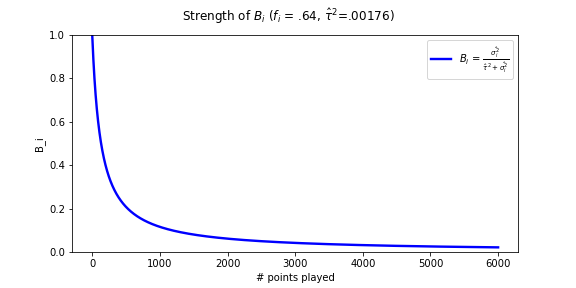
\includegraphics[scale=.7]{norm_fig}


%If Machado were to have lost against Tursunov, then our cross entropy would increase by $\approx 22$, a huge penalty for a single data point. Given Tursunov's elo advantage, this is not a situation to which we want to expose models forecasting. In the end, the James-Stein estimator offers robustness to serve/return probabilities derived from infrequently charted players. We will hold onto these estimates for use in future models.

\section{Opponent-Adjusted Serve/Return Statistics}

While Barnette and Clarke's equation does consider opponent's serve and return ability, it does not track average opponents' ability within a player's history. This is important, as a player's serve/return percentages may become inflated from playing weaker opponents or vice versa. In this section, we propose a variation to Barnette and Clarke's equation which replaces $f_{av},g_{av}$ with opponent-adjusted averages $1-g_{i\_opp\_av},1-f_{i\_opp\_av}$ for $p_i$. The equations then become:

\begin{center}
$f_{ij} = f_t + (f_i-(1-g_{i\_opp\_av}))-(g_j-(1-f_{j\_opp\_av}))$
%\newline
$f_{ji} = f_t + (f_j-(1-g_{j\_opp\_av}))-(g_i-(1-f_{i\_opp\_av}))$
\end{center}

$g_{i\_opp\_av}$ represents the average return ability of opponents that $p_i$ has faced in the last twelve months. To calculate this, we weight each opponent's return ability $g_j$ by number of points in their respective match.

$g_{i\_opp\_av} = \frac{\sum_{t=1}^{12}\sum_{k \in (i,y-1,m+t)}{\text{(\# of $p_i$'s return points in match k)*($p_j$'s return ability before match k)}}}{\sum_{t=1}^{12}\sum_{k \in (i,y-1,m+t)}\text{\# of $p_i$'s return points in match k}}$

To illustrate the effect of tracking opponent-adjusted statistics, we consider the 2014 US Open first-round match between Mikhail Youzhny (RUS) and Nick Kyrgios  (AUS).

\makebox[\textwidth][c]{\begin{tabular}{ |c|c|c|c|c|c|c|c| }
 \hline
 player name & s\_points\_won & s\_points
 & $f_i$ & r\_points\_won & r\_points & $g_i$ & elo rating \\ 
 \hline
 Mikhail Youzhny & 1828 & 2960 & .6176 & 1145 & 2947 & .3885 & 1749.77
 \\
 \hline
 Nick Kyrgios & 900 & 1370 & .6569 & 424 & 1323 & .3205 & 1645.03 \\ 
 \hline
\end{tabular}}

From the standard approach, with $f_t =.6583$, we compute $f_{ij} = .6446, f_{ji} = .6159$. Then, to calculated adjusted statistics, we consider the expected number of points won on serve/return, given Youzhny and Kyrgios' past opponents. As we can observe from $f_{i\_opp\_av},g_{i\_opp\_av}$, Kyrgios has faced faced slightly stronger opponents than Youzhny over the past twelve months.

\makebox[\textwidth][c]{\begin{tabular}{ |c|c|c|c|c|c|c| } 
 \hline
 player name & $g_{i\_opp\_av}$ & s\_expected
& s\_adj & $f_{i\_opp\_av}$ & r\_expected & r\_adj  \\ 
 \hline
 Mikhail Youzhny & .4156 & 1729.74 & .0332 & .6812 & 939.60 & .0697
 \\
 \hline
 Nick Kyrgios & .4313  & 779.19 & .0882 & .7060 & 388.92 & .0265  \\ 
 \hline
\end{tabular}}

%\makebox[\textwidth][c]{\begin{tabular}{ |c|c|c|c|c|c|c| } \hline player name & $g_{i\_opp\_av}$ & s\_expected & s\_adj & $f_{i\_opp\_av}$ & r\_expected & r\_adj  \\ \hline Mikhail Youzhny & .4156 & 1729.74 & .0332 & .6812 & 939.60 & .0697 \\ \hline Nick Kyrgios & .4313  & 779.19 & .0882 & .7060 & 388.92 & .0265  \\  \hline \end{tabular}}


$s_{adj\_i}, r_{adj\_i}$, and adjusted serve probabilities $adj(f_{ij}),adj(f_{ji})$ are calculated as follows:

$s_{adj\_i} = \frac{\text{\# points won on serve}}{\text{\# points on serve}} - (1-g_{i\_opp\_av}) = f_i-(1-g_{i\_opp\_av}) \newline r_{adj\_i} = \frac{\text{\# points won on return}}{\text{\# points on return}} - (1-f_{i\_opp\_av}) = g_i-(1-f_{i\_opp\_av})
\newline adj(f_{ij}) = f_t + (f_i-(1-g_{i\_opp\_av}))-(g_j-(1-f_{j\_opp\_av})) = f_t + s_{adj\_i} - r_{adj\_j} = .6288
\newline adj(f_{ji}) = f_t + (f_j-(1-g_{j\_opp\_av}))-(g_i-(1-f_{i\_opp\_av})) = f_t + s_{adj\_j} - r_{adj\_i} = .6406$

Using regular serve probabilities, Youzhny is favored to win with $P_m(0,0,0,0,0,0)=.6410$. With adjusted serving percentages, we factor in the stronger opponents in Kyrgios' match history and Youzhny's win probability drops to $M_p(0,0,0,0,0,0) = .4411$. While adjusted serve/return statistics do not always cause significant shifts in win probability, they consistently account for relative ability of players' opponents in producing serve probabilities $f_{ij},f_{ji}$.  

\section{Results}
The following results were obtained using ATP best-of-three matches in our point-by-point dataset, excluding Davis Cup.\footnote{The Davis Cup is a year-long competition between teams organized by country. Since Kovalchik excluded Davis Cup matches from her evaluation \citep{Kovalchik2016} and many match-ups involve relatively unknown players, we exclude all matches.} We observe performance across variants of elo-based predictions and point-based models. Since all original implementations provide explicit formulas with no optimization, we directly assess their performance on 2014 tour-level data (2,409 matches). In the case of logistic regression, the model was trained on tour-level data from 2011-2013 (7,828 matches). We measure each model's performance in terms of accuracy, as in section 3.3. We also consider log loss, a measure of overall likelihood of a model's predictions. Log loss is important because it penalizes models that incorrectly assign over-confident or under-confident win probabilities. As we are hoping to optimize in-match prediction models' log loss, it is important to consider the likelihood of various pre-match forecasts. The following terms express variations to point-based and Elo models:

\setlist[description]{leftmargin=\parindent, labelindent=\parindent}
\begin{description}[leftmargin=2.5cm, labelindent=2.5cm]
\item[KM] - point-based hierarchical Markov models with combined serve/return percentages from Barnett/Clarke

\item[James-Stein] - version of a KM model, with all serve/return percentages normalized with James-Stein estimator

\item[surface] - version of model where all ratings and percentages are stratified by surface (Hard, Clay, Grass)

\item[538] - specifically denotes Five-Thirty-Eight's ``decaying $k$-factor'' method in computing Elo ratings
\end{description}

\begin{center}
\begin{table}[H]
        \caption{Results Table}
        \centering
        \begin{tabular}{@{}clcc@{}}
            \toprule
            Method & Variation & Accuracy & Log Loss \\\midrule

            KM & & 64.8 & .649  \\\addlinespace
            
            KM & James-Stein & 65.4 & .616
  \\\addlinespace
 KM & surface & 63.3 & .707
  \\\addlinespace
 KM & surface James-Stein & 63.6 & .639 \\\addlinespace
 KM & adjusted & 67.8 & .632 \\\addlinespace
 KM & adjusted James-Stein & 67.9 & .617 \\\addlinespace
 Elo &  & 69.1 & .586 \\\addlinespace
 Elo & surface & 68.4 & .591 \\\addlinespace
 Elo & 538 & 69.2 & .587 \\\addlinespace
 Elo & surface 538 & 69.4 & .592 \\\addlinespace
 Logit & Elo 538, surface Elo 538 & 69.5 & .577 \\\addlinespace
            \bottomrule
        \end{tabular}
    \end{table}
    \end{center}

\subsection{Discussion}

As expected, James-Stein normalization significantly improves each point-based model's log loss. While surface-based Elo is competitive with regular elo, restricting Klaassen and Magnus' point-based method to surface-specific data clearly hurts performance. This is presumably due to limited surface-specific data. As many players perform differently across surfaces, computing serve percentages from surface-specific data offers the potential to express how players' performance varies by surface. Yet, even with James-Stein normalization, the loss in sample size appears to outweigh the benefits obtained from surface-specific data. As we did not rigorously explore possibilities for weighting players' surface-specific statistics, there may still be potential for a point-based model that effectively considers surface in computing serve/return percentages. Finally, using opponent-adjusted serve-return statistics further improved performance. By fully incorporating each opponent's ability in a player's match history, this model approached Elo ratings in likeness of predictions, with win-probability forecasts between the two sharing $R^2=.76$.

By plugging Elo and surface Elo into a logistic regression model, we achieve a log loss of .577. After fitting to the training data, this model learned coefficients for each variable that assigned a 56\% weight to regular Elo ratings and 44\% weight to surface Elo ratings. The near-even weight to both types of ratings suggests how important surface-specific ability is toward forecasting matches. Aside from models which draw information directly from the betting market, no other model has documented preferable log loss. Kovalchik reported 70$\%$ accuracy using 538's Elo method \citep{Kovalchik2016}, calculating Elo ratings using satellite events (ATP Challengers and Futures) in addition to tour-level events \footnote{One can observe at https://github.com/skoval/deuce.}. While this accounted for a small increase in accuracy, her method achieved a log loss of .59, which does not outperform our implementation. For simplicity's sake, we calculated all Elo ratings and statistics from tour-level matches alone.\footnote{There are about 3,000 tour-level matches each year.} In the end, our Elo-based logistic regression's incremental improvement over singular Elo ratings implies that an effective rating system should consider a overall ability as well as surface-specific ability.


%holds several implications. First, there is useful information about players contained in both surface-specific and non-surface Elo ratings. Second, models that do not draw information from the betting market, no other tennis-specific methods have charted better performance \cite{Kovalchik2016}. 

%(you can attempt to combine both Elo ratings with Gaussian processes or the hyperparameter hack)

Sipko recently explored machine-learning methods for pre-match prediction, surveying logistic regression, the common-opponent model, and an artificial neural net \citep{Sipko2015}. While he claimed to have achieved 4.3$\%$ return-on-investment off the betting market with an artificial neural net, his machine learning models did not beat a log loss of .61 when predicting 2013-2014 ATP matches\footnote{The models were trained on 2004-2010 ATP matches and validated on 2011-2012 ATP matches.}. Despite the current deep-learning craze throughout industry and academia \citep{lewis2016great}, no one has published findings to suggest their superiority in predicting tennis matches. Short of market-based models, it appears most effective to stick with elo's ``ruthlessly Bayesian design'' which FiveThirtyEight so frequently touts \citep{HowForecasting}. Transitioning onward, we will consider how these findings may inform an effective in-match prediction model.


%As Sipko surveyed logistic regression, the common-opponent model, and an artificial neural net, we are confident that Elo provides a confident starting place for in-match prediction models.

%The question becomes, how can this serve our in-match predictions?

%It is important to note that Klaassen and Magnus' method of combining player statistics involves no optimization with respect to a training dataset. Of the above methods, only a logistic regression with Elo and surface Elo actually learns its model parameters with respect to a training dataset. 



\chapter{In-game Match Prediction}

%Having surveyed all relevant pre-match prediction models, we proceed to in-match prediction. 

The following methods will be tested on tour-level matches for which we have point-by-point data. The matches span 2010-2017, accounting for nearly half of all tour-level matches within this time. Point-by-point records in Sackmann's dataset take the form of the following string:

Mikhail Youzhny vs. Evgeny Donskoy (Australian Open 2013, Round 2)

P=\seqsplit{``$SSRSS; RRRR; SRSSS; SRRSRSSS; SRSSRS; RSRSSS; SRSRSS; RSRSRSSS; SSSS. SSSRRRSS; RSSSS; SSRSS; SSSRS; SSSS; RRRSSSSRRSSRRSRSSS; SRSRSS; SSSRS; RSRSSRSS; SSSS; SRSSS; RSRSSRRSSS; R/ SR/ SS/ RR/ RS/SR. RSRRR ;...$''}

%P=\seqsplit{``$SSRSS;RRRR;SRSSS;SRRSRSSS;SRSSRS;RSRSSS;SRSRSS;RSRSRSSS;SSSS.SSSRRRSS;RSSSS;SSRSS;SSSRS;SSSS;RRRSSSSRRSSRRSRSSS;SRSRSS;SSSRS;RSRSSRSS;SSSS;SRSSS;RSRSSRRSSS;R/SR/SS/RR/RS/SR.RSRRR;...$''}

$S$ denotes a point won by the server and $R$ a point won by the returner. Individual games are separated by ``$;$'', sets by ``$.$'', and service changes in tiebreaks by ``$/$''. By iterating through the string, one can construct $n$ data points $\{P_0,P_1,...,P_{n-1}\}$ from a match with $n$ total points, with $P_i$ representing the subset of the match after which $i$ points have been played.

$P_0 = ``"$

$P_1 = ``S"$

$P_2 = ``SS"$

$P_3 = ``SSR"$

...

With $M = \{M_1,M_2,...M_k\}$ representing complete match-strings in our point-by-point dataset, the size of our enumerated dataset becomes $\sum_{i=1}^k |M_i|$. In total, this sums to over 1.2 million individual points within ATP matches spanning 2010-2017. While many in-match prediction models utilize the hierarchical Markov Model structure, we will first test several machine-learning methods as a baseline. Now, we will explore the following methods:

\begin{itemize}
  \item Logistic Regression
  \item Random Forests
  \item Hierarchical Markov Model
  \item Beta Experiments 
  \item Elo-induced Serve percentages
\end{itemize}

%we may apply serving percentages from the past section to in-match prediction. To start, 

\section{Logistic Regression}
%$logit(x_i)$ yields $p_i$'s win probability from input $x_i$.

Consider a Logistic Regression model where each observation $x_i = [x_{i1},x_{i2},...,x_{ik}]$ has $k$ features. When $P$ represents $p_i$'s win probability,

$$ \log{\tfrac{P}{1-P}} = \beta_0+\beta_1(x_{i1})+\beta_2(x_{i2})+...+\beta_k(x_{ik})$$

%$$P = \frac{1}{1+e^{-(\beta_0+\beta_1(x_{i1})+\beta_1(x_{i2})+...+\beta_1(x_{ik}))}}$$

From any scoreline ($s_i,s_j,g_i,g_j,{x}_i,{x}_j$), we can simply feed these values into our model as features of $x_i$. Logistic Regression's structure makes it easy to consider additional features for each player, such as Elo difference, surface Elo difference, or break advantage. Before adding more features to the model, we consider two baselines: a model using score differentials ($s_i-s_j,g_i-g_j,{x}_i-{x}_j$) and another model trained on Elo differences and lead heuristic $L_{ij}$. This heuristic estimates $p_i$'s total lead in sets, games, and points:

\begin{center}
$L_{ij} = (s_i-s_j) + \frac{1}{6}(g_i-g_j) + \frac{1}{24}(x_i-x_j)$
\end{center}

The coefficients preserve order between sets, games, and points, as one cannot lead by six games without winning a set or four points without winning a game. While it assumes these relative orderings, the heuristic is meant to approximate how much $p_i$ leads $p_j$ from any scoreline. In this model, we consider the following features in predicting the winner of the match:

\begin{table}[H]
\centering
\caption{Logistic Regression Features}
\label{my-label}
\begin{tabular}{ll}
 \hline
 $Variable$ & $Description$ \\
 \hline
 lead\_margin & lead heuristic $L_{ij}$ \\
 \hline
 eloDiff &  Elo($p_0$) - Elo($p_1$) \\
 \hline
  s\_eloDiff &  s\_Elo($p_0$) - s\_Elo($p_1$) \\
 \hline
 setDiff &  SetsWon($p_0$) - SetsWon($p_1$)\\
 \hline
 gameDiff &  inSetGamesWon($p_0$) - inSetGamesWon($p_1$)\\
 \hline
 pointDiff &  inGamePointsWon($p_0$) - inGamePointsWon($p_1$)\\
 \hline
  breakAdv &  ServeGamesWon($p_0$) - ServeGamesWon($p_1$) + I(currently serving)\\
 \hline
 brkPointAdv & I(holding break point) - I(facing break point)\\
 \hline
 sv\_points\_pct\_0 & percentage of points won on $p_0$'s serve thus far\\
 \hline
 sv\_points\_pct\_1 & percentage of points won on $p_1$'s serve thus far\\
 \hline
\end{tabular}
\end{table}

Next, we test the following combinations of features:

1) setDiff + gameDiff + pointDiff (Differentials)

2) lead\_margin + eloDiff + s\_eloDiff (Elo)

3) all features (All)

\subsection{Cross Validation}

Each match in our best-of-three dataset has around 160 points on average. In tuning hyper parameters for machine learning models, we implement $k$-fold group validation with $k=5$. This randomly splits the training set into five subsets of roughly equal size, while always grouping points from the same match in the same fold. By grouping points from the same match together, this method prevents overlap across train, validation, and test sets. Treating each subset as a validation set, we train all models on the remaining data before testing performance on the corresponding validation set. Then we average performance across all $k$ validation sets and select the hyper parameters whose models performed best. When we assess model performance on validation and test sets, results then reflect performance on matches a model has never seen before. 

%prevents information within a single match from informing the model before we test performance on other points from the same match. 

%(actually didn't do hyperparameter cross-validation because it seemed unnecessary...)

%\subsection{Visualizing Logistic Regression ??? here???}


%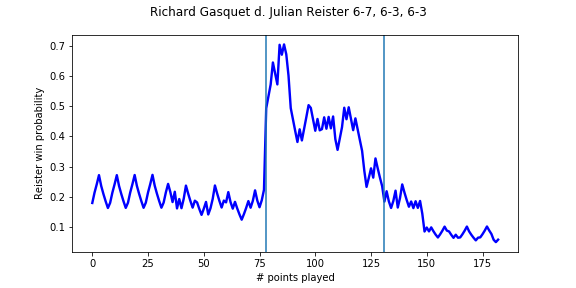
\includegraphics[scale=.7]{gasquet_reister_9_6_all_features}

%One drawback of logistic regression is that it cannot distinguish between situations whose score differentials are equivalent. A player serving at (1,1),(5,4),(3,0) will have approximately the same win probability as one serving at (1,1),(1,0),(3,0). However, in the first situation, the player serving wins the match if he wins any of the next three points. From the second scenario, the player serving only holds a break advantage early in the set, from which the returner has many more chances to come back. Assuming each player serves at $f_i=f_j=.64$, our win-probability equation suggests a substantial difference between these two scenarios:

%\begin{center}
%$P_m(1,1,5,4,3,0) = .994$

%$P_m(1,1,1,0,3,0) = .800$
%\end{center}

%Although the first situation is clearly favorable, logistic regression will compute approximately the same probability in both scenarios $\footnote{\text{after fitting coefficients for the equation P(win) = logit($s_i,s_j,g_i,g_j,{x}_i,{x}_j)= \frac{e^{(c_1s_i+c_2s_j+c_3g_i+c_4g_j+c_5x_i+c_6x_j}}{1+e^{(c_1s_i+c_2s_j+c_3g_i+c_4g_j+c_5x_i+c_6x_j}}$}, coefficients $ c_1 \approx c_2, c_3 \approx c_4,c_5 \approx c_6$ by symmetry and therefore $logit(1,0,5,4,3,0) \approx logit(1,0,1,0,3,0) $}$

%$\footnote{after fitting coefficients for the equation $P(win) = logit(s_i,s_j,g_i,g_j,{x}_i,{x}_j) = \frac{e^{(c_1s_i+c_2s_j+c_3g_i+c_4g_j+c_5x_i+c_6x_j}}{55}$, coefficients $ c_1 \approx c_2, c_3 \approx c_4,c_5 \approx c_6$ by symmetry and therefore}$

%Another issue is that logistic regression can fail to detect when a higher-ranked player is about to lose in a close match. Below,

%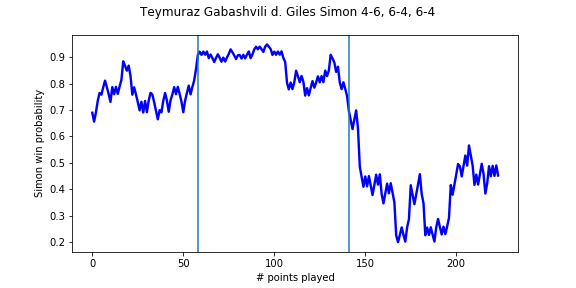
\includegraphics[scale=.7]{simon_gabashvili_9_6_all_features}

%Simon leads for most of the match until Gabashvili comes back to force the third set. At the end of the third set, Gabashvili serves out the match from 5-4, yet the model fails to detect that Simon is about to lose. This is because, with sets at 1-1 and game differentials nearly even, Simon's Elo advantage outweighs his current scoreline disadvantage. Consequentially, his win-probability hovers between 40-50\% as he loses the match, rather than fall toward 0.


\section{Random Forests}
Brian Burke's win-probability models are among the most well-known in sports \citep{WPexp}. They calculate a team's win probability at any point in the match based on historical data through a combination of binning inputs and smoothing their resulting probabilities. Nettleton and Lock built on this method by using a Random Forest approach \citep{LockandNettleton2014}.

A Random Forest consists of an ensemble of randomly generated classification trees. Each tree forms decision functions for a subset of features with splits that generate maximum discriminatory ability. As Nettleton and Lock do so with football-specific features such as down, points, and yards to goal, we do so with analogous tennis features and train on our validation set.

%Nettleton and Lock also deviate from the traditional random forest classification problem in using regression trees and averaging their estimates to produce a probability estimate, rather than a majority vote.

%Then, training on our validation set, we test two random forest models on our point-by-point dataset, one with classification trees and one with regression trees.

\begin{table}[H]
\centering
\caption{Random Forest features}
\label{my-label}
\begin{tabular}{ll}
 \hline
 Variable & Description \\
 \hline
 surface & hard, clay, grass \\
 \hline
 set &  first, second, third \\
 \hline
 eloDiff &  Elo($p_0$) - Elo($p_1$) \\
 \hline
  setDiff &  SetsWon($p_0$) - SetsWon($p_1$)\\
 \hline
 gameDiff &  inSetGamesWon($p_0$) - inSetGamesWon($p_1$)\\
 \hline
 pointDiff &  inGamePointsWon($p_0$) - inGamePointsWon($p_1$)\\
 \hline
  breakAdv &  ServeGamesWon($p_0$) - ServeGamesWon($p_1$) + I(currently serving)\\
 \hline
 brkPointAdv & I(holding break point) - I(facing break point)\\
 \hline
\end{tabular}
\end{table}

\section{Hierarchical Markov Model}
With serving percentages already calculated from historical data, our hierarchical Markov model is well-equipped to produce in-match win probability estimates. Using the analytical equation with players' serving abilities $f_{ij},f_{ji}$, we compute $P_m(s_i,s_j,g_i,g_j,x_i,x_j)$ from every scoreline $(s_i,s_j,g_i,g_j,x_i,x_j)$ in a match. To assess this model's performance, we repeat this on every match in our dataset, with $f_{ij},f_{ji}$ computed with one's method of choice.

\subsection{Beta Experiments}
The above approach only takes into account the current score and pre-calculated serve percentages when computing win probability. However, in many cases, relevant information may be collected from $P_k$. Consider the following in-match substring, 

$P=``SSSS;RSSSRRSS;SSSS;SRRSRSRSSS;SSSS;RRRSSSRSRSSS;"$

The above sequence demonstrates a current scoreline of three games all. However, $p_i$ has won 12/12 service points, while $p_j$ has won 18/30 service points. If both players continue serving at similar rates, $p_i$ is much more likely to break serve and win the match. Since original forecasts $f_{ij},f_{ji}$ are based on historical serving percentages, it makes sense that in-match serving percentages may help us better determine each player's serving ability on a given day. To do this, we can update $f_{ij},f_{ji}$ at time $t$ of the match to factor in each player's serving performance thus far.

Bevc explored this method by modeling each player's serving percentage $f_{ij}$ with a beta prior $b_{prior}$ that could be updated mid-match to yield posterior estimates. Through beta-binomial conjugacy, we can update $b_{prior}$ when a player has won $s_{won}$ points on serve out of $s_{total}$ trials.

\begin{center}
$b_{prior} \sim \text{Beta}(a,b)$ 

$b_{posterior} \sim \text{Beta}(a+s_{won},b+s_{total}-s_{won})$
\end{center}

%The beta distribution is a generalization of the uniform distribution. We often use the beta distribution to represent prior and posterior estimates of some unknown probability $p$. (can include stats notation with beta-binomial conjugacy)

If $f_{ij}$ is our prior, $a,b$ must satisfy $E(b_{prior}) = \frac{a}{a+b} = f_{ij}$. Then $a$ is a hyperparameter that determines the strength of our prior. To find a suitable prior strength, we will test various values of $a$ via cross-validation on our training set. Regardless of $a$, the match's influence on our posterior serve estimates always grows as more points have been played. At any point in the match, we can always obtain a posterior serving percentage for either player of the form

$f_{ij}' = E(b_{posterior}) = \dfrac{a + s_{won}}{a + b + s_{total}}$


%To update our matches with in-match serving statistics, we set $f_{ij}$ as a prior and update with the number of points won and played on $p_i's$ serve, $(s_{won},s_{pt})$. 

\subsection{Elo-induced Serve Probabilities}
Earlier on, Klaassen and Magnus suggested a method to infer serving probabilities from a pre-match win forecast $\pi_{ij}$. By imposing a constraint $f_{ij}+f_{ji}=t$, we can then create a one-to-one function 
$S: S(\pi_{ij},t) \rightarrow (f_i,f_j)$, which generates serving probabilities $\hat{f_{ij}},\hat{f_{ji}}$ for both players such that $P_{m}(0,0,0,0,0,0)=\pi_{ij}$.\footnote{$f_{ij}$ and $f_{ji}$ are computed as specified in 3.4 with James-Stein normalization, so as to prevent extreme results.} As this paper was published in 2002, Klaassen and Magnus inverted their match probability equations to produce serve probabilities for ATP rank-based forecasts. However, since Elo outperforms ATP rank, we apply this method to Elo forecasts.

Due to branching complexity (see section 2.5), our hierarchical Markov model's match probability equation has no analytical solution to its inverse, even when we specify $f_{ij}+f_{ji}=t$. Therefore, we turn to the following approximation algorithm to generate serving percentages that correspond to a win probability within $\epsilon$ of our Elo forecast's:

\begin{algorithm}[H]
\caption{elo-induced serve probabilities}\label{euclid}
\begin{algorithmic}[H]
\Procedure{EloInducedServe(prob,sum,$\epsilon$)}{}
\State $\text{s0} \gets \text{sum/2}$
\State $\text{currentProb} \gets \text{.5}$
\State $\text{diff} \gets \text{sum/4}$

\While {$|$currentProb - prob$| > \epsilon $}:

\If {$\text{currentProb \textless$ $ prob}$}
\State s0 += diff 
\Else
\State s0 -= diff
\EndIf
\State diff = diff/2
\State $\text{currentProb} \gets \text{matchProb(s0,sum-s0)}$

\EndWhile


\State \Return s0, sum-s0

\EndProcedure
\end{algorithmic}
\end{algorithm}

To generate elo-induced serve probabilities for a given match, we run the above algorithm with PROB=$\pi_{ij}$, SUM=$f_{ij}+f_{ji}$, and $\epsilon$ set to a desired precision level.$\footnote{For purposes of this project, setting $epsilon$=.001 is sufficiently accurate.}$ At each step, we call matchProb() to compute the win probability from the start of the match if $p_i$ and $p_j$ had serve probabilities $f_{ij}=s0, f_{ji}=\text{sum}-s0$, respectively. Then we compare currentProb to prob and increment s0 by diff, which halves at every iteration. This process continues until the serve probabilities s0, sum-s0 produce a win probability within $\epsilon$ of PROB, taking $O(\log{\frac{1}{\epsilon}})$ calls to matchProb.

This inverse algorithm is useful for several reasons. Given any effective pre-match forecast $\pi_{ij}$, we can produce serve probabilities that are consistent with $\pi_{ij}$ according to our hierarchical Markov model. By setting the constraint $f_{ij}+f_{ji}=t$, we also ensure that the sum of our players' serve probabilities agrees with historical data. \footnote{While it is just an estimate, $t=f_{ij}+f_{ji}$ is our best predictor of overall serving ability from methods covered in this project.} While Klaassen and Magnus argue that $t = f_{ij}+f_{ji}$ is largely independent of $\pi_{ij}$, $t$ holds greater importance when predicting specific scorelines a match \citep{Barnett2006}. Using the hierarchical Markov Model's equations, Barnette specifically computed the probability of reaching any set score given $f_{ij},f_{ji}$. When comparing probabilities across matches, one can observe that as $t$ increases, closer set scores and tiebreak games become more likely.\footnote{7-6, 6-7, 7-5, 5-7, etc.} That is, $t$ encodes information regarding likely trajectories of a match scoreline and relative importance of winning each game on serve. For higher $t$, service games are won more often and service breaks hold relatively more importance, while the opposite holds for lower $t$. Now, given $\pi_{ij}$ and $t$, we can produce elo-induced serve probabilities for any two players.

%\footnote{to avoid extreme values of $t$ from limited player data, we use James-Stein normalized estimates to calculate $t$: $t = JS(f_{ij})+JS(f_{ji})$}



\subsection{Importance of $f_{ij}+f_{ji}$}

To illustrate the importance of $t=f_{ij}+f_{ji}$, we consider the two following matches:

\begin{center}
\begin{tabular}{ |c|c|c|c|c|c|c| } 
 \hline
 match & $p_i$ & $p_j$ & tny\_name & surface
 & $\pi_{ij}$ & $t$ \\ 
 \hline
 $m_1$ & Feliciano Lopez & John Isner & ATP Shanghai 2014 & hard & .478 & 1.55 \\
 \hline
  $m_2$ & Andreas Seppi & Juan Monaco & ATP Kitzb$\ddot{\text{u}}$hel 2014 & clay & .476 & 1.14
 \\
 \hline

\end{tabular}
\end{center}

In both matches, $\pi_{ij}$ is approximately the same while $t$ differs significantly. To visualize how service breaks can have varying importance, consider win-probability graphs corresponding to the following progression of points, $P$. In each scenario, $p_i$ and $p_j$'s serve probabilities are calculated from method 4.3.2.

$P=``SSSS;SSSS;SSSS;SSSS;SSSS;RRRR"$

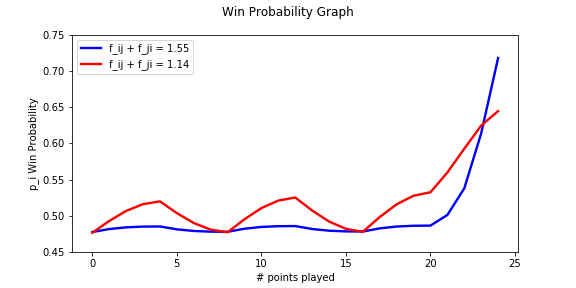
\includegraphics[scale=.7]{m12_wp}

Over the first five games, both players win every point on serve. When $t=1.55$, service holds are expected and and win probability hardly moves. After $p_i$ breaks serve in the sixth game, his win probability suddenly spikes up, indicating a substantial advantage. When $t=1.14$, our model assumes that players win service games with much lower probability. Therefore, each time a player holds serve, his win probability noticeably increases. When $p_i$ breaks in the sixth game, his win probability climbs, but not as dramatically as in the previous case. When service games are won at a lower probability, service break advantages become weaker.

$t$'s influence on the trajectory of a match suggests that prediction from any in-match scoreline will be most effective when $t$ accurately reflects the players' overall serving ability. While Elo ratings or betting odds yield the most effective pre-match predictions \citep{Kovalchik2016}, their implied odds offer no information about $t$ in a given match-up. As $t$ holds significance for in-match forecasting from specific scorelines, method 4.3.2 allows us to combine any effective pre-match forecast $\pi_{ij}$ with $t$ to produce new serving probabilities.

%To preserve information about the shape of each match, we set the constraint $t = f_{ij}+f_{ji}$, rather than some constant $k = f_{av}+g_{av}$.

%Examples: Federer vs Isner at Paris (or Karlovic vs Isner for more even match), then Ferrer vs. Nishikori/Schwartzman or something with really good returners. (can visualize this with new win probabilities, use example when Karlovic and Schwartzman both had the same win probability)

% write about importance on shape of match


%Take two matches with $\pi_{1ij} \approx \pi_{2ij}$. Then graph the matches' WP with respect to a made-up scoreline that includes one service break.

%Since Elo ratings fail to capture this, it is crucial that we find a way to incorporate this into our model.

%show a histogram of $t$ (?):

\section{Results}

The following models were trained on 2011-2013 point-by-point data (4584 matches) and tested on 2014 point-by-point data (1855 matches). For consistency, we only used best-of-three ATP tour-level matches and excluded matches from the Davis Cup. From cross-validation on the training set, we determined that setting hyper-parameter $a=300$ yielded optimal performance across beta experiments. We then added a beta variation to KM elo-induced and KM logit-induced, our two best-performing point-based models. As observations corresponds to a single point in each match, longer matches contribute more to our dataset and have larger influence on evaluation metrics. Since addressing this outsized influence could complicate results' interpretability, we present model evaluation on a point-by-point basis.

\setlist[description]{leftmargin=\parindent, labelindent=\parindent}
\begin{description}[leftmargin=1.7cm, labelindent=1.7cm]
\item[LR] - Logistic Regression model with feature set specified in 4.1

\item[RF] - Random Forest model with feature set specified in 4.2

\item[Equivalent] - KM model with serve probabilities set to tour-level averages (assumes equal player ability)

\item[elo-induced] - KM model with serve probabilities generated from elo-based win probability

\item[logit-elo] - KM model with serve probabilities generated from logistic regression on Elo and surface-based elo
\end{description}





\begin{center}
\begin{table}[H]
        \caption{Results Table}
        \centering
        \begin{tabular}{@{}clccc@{}}
            \toprule
            Method & Variation & Accuracy & Log Loss & Calibration \\\midrule

            LR & Differentials & 71.4 & .540 & .993  \\\addlinespace
            
            LR & Elo & 75.2 & .505 & 1.006
  \\\addlinespace
 LR & All & 76.2 & .488 & .993
  \\\addlinespace
 RF &  & 70.1 & .562 & .902\\\addlinespace
 KM & Equivalent & 71.5 & .538 & 1.040\\\addlinespace
 KM & James-Stein & 74.9 & .501 & 1.002\\\addlinespace
 KM & adjusted James-Stein & 75.9 & .498 & .992\\\addlinespace
 KM & elo-induced & 76.2 & .486 & 1.001\\\addlinespace
 KM & elo-induced (a=300) & 76.3 & .481 & 1.003\\\addlinespace
 KM & logit-elo & 76.5 & .481 & .996\\\addlinespace
 KM & logit-elo (a=300) & 76.5 & .477 & .999\\\addlinespace
            \bottomrule
        \end{tabular}
    \end{table}
    \end{center}

Of our models, Random Forest had the least predictive power. While this is perhaps due to difficulty in constructing an effective feature space, nearly all features fed into each machine learning model had an additive effect on win probability. Positive score differentials, break advantages, and elo differences will all boost a player's expected win probability. The only non-additive features considered were ``set'' and ``surface.'' While the random forest model was able to consider various situations among these two features, we conclude that its inclination to group similar examples together, rather than estimate linear relationships between variables, ultimately accounted for its performance.

%point out how we tried LR with interaction but didn't see much improvement

Logistic Regression, on the other hand, is designed to  learn additive relationships between features and its probability output. It's performance with the full feature set was competitive with our point-based models, despite their superior grasp of tennis' scoring system.\footnote{Consider, for example, how logistic regression has no knowledge of when tiebreak games occur.} Presumably, this model holds an advantage over point-based models in its ability to fit itself to the training data. Aside from our hyper-parameter search of $a$ in beta experiments, the point-based models offer no comparable method to optimize performance with respect to a training set.

%When we consider prediction models for tennis, we want the following condition to hold: for any score line $(s_i,s_j,g_i,g_j,{x}_i,{x}_j)$, a suitable model with formula $P_m$ should produce win probability such that $P_m(s_i,s_j,g_i,g_j,{x}_i+1,{x}_j) > P_m(s_i,s_j,g_i,g_j,{x}_i,{x}_j)$. That is, at any stage in the match, $p_i$'s win probability should always increase after winning the next point. While there are no guarantees of maintaining this property with machine learning models, our point-based model will satisfy this condition without fail. \footnote{section 2.5 verifies this}

Of the point-based models, KM logit-elo (a=300) achieved the best performance, although the improvement from running beta experiments was marginal. Since Elo ratings produce more reliable pre-match win forecasts $\pi_{ij}$ than estimates of $f_{ij},f_{ji}$ from historical serve/return data, using serve probabilities induced from elo ratings and then from our logit Elo model improved our models performance by significant increments. Over the next few sections, we will examine our models' calibration and performance across subsets of our dataset.

%Interestingly, logistic regression with our complete feature set performed nearly as well as our best variation of the KM point-based model. Despite issues discussed in 4.1.2, logistic regression can still perform nearly as well ase the best of our point-based models.

\subsection{Model Calibration}

\hspace*{-.5cm}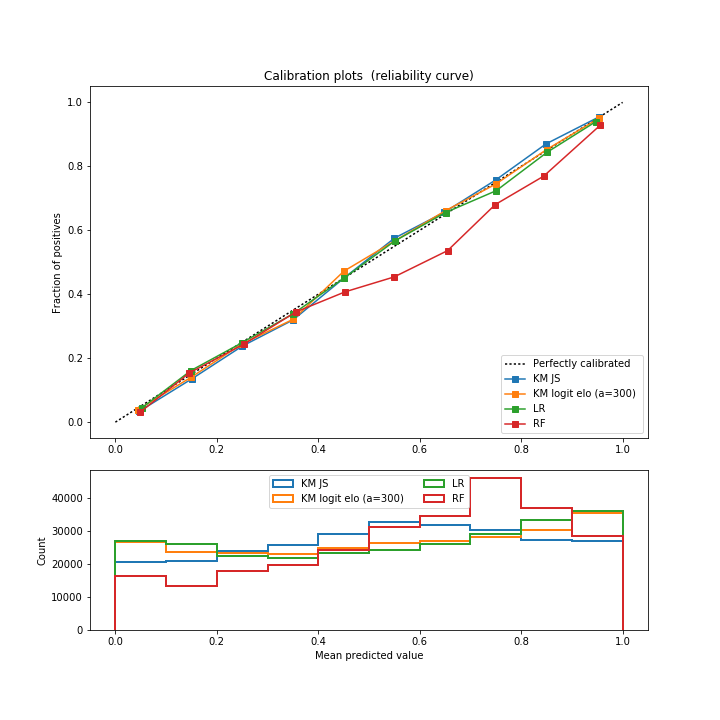
\includegraphics[scale=.6]{calibration_plot}

Calibration represents the ratio between observed rate of success and mean predicted rate of success. From a perfectly calibrated model that predicts a win probability of $p$, we can always expect a win to occur with probability $p$. While the Random Forest model under-predicted wins, the rest of our models closely resemble a perfectly calibrated model. From our table, KM logit elo and KM JS exhibited near-perfect calibration of 1.001 and .999, while Logistic Regression reported .993. As there is degree of uncertainty in measuring calibration, we could not reasonably expect to produce more well-calibrated models. Given win probability forecast $\pi_{ij}$ at any point of a match within our test set, we expect $p_i$ to win with probability $\pi_{ij}$.

\subsection{By Set}

%to do: display uncertainty lines on each bar?? not sure if this is meaningful?

\hspace*{-1.5cm}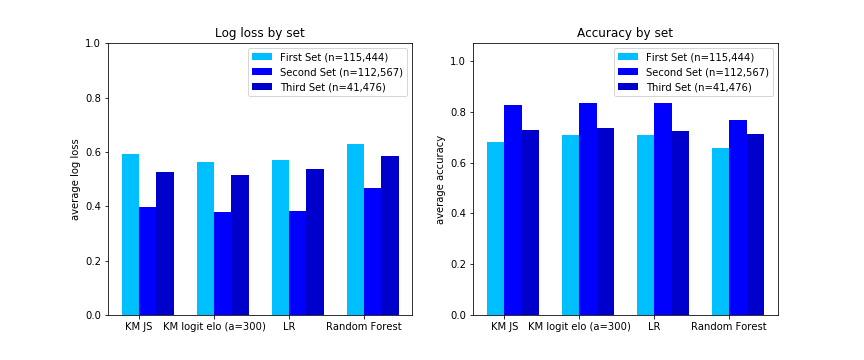
\includegraphics[scale=.6]{set_performance3}

Since we have less information about a match early on, it is always most difficult to forecast matches during the first set. However, across both metrics, models are most effective during the second set. By this time in the match, the winner of the first set is often a clear favorite to win the match, unless their opponent has a significantly higher Elo rating or serve percentage $f_{ji}$. As 64.3\% of matches in our test set are straight-sets victories, many matches offer relatively easy predictions for our model during the second set.\footnote{Best-of-three matches that end in two sets are straight-sets.}

Uncertainty increases once the match enters a third set because the set score has evened at 1-1. While the set score is tied in both first and third sets, it is easier to predict the outcome during the third set because its outcome corresponds directly to the match outcome. When predicting in the first set, the player who wins the first set can still go on to lose the match, which increases uncertainty.

%If we are equally confident in predicting P(win current set) across all sets, then P(win | current set) = 1 in third set while P(win | current set) is less certain in the first set. Discuss how performance differs by set (1st, 2nd, 3rd) From a favorable position in the third set, one is more likely to win the match since winning the first set does not clinch the match.

\subsection{By Surface}

\hspace*{-1.5cm}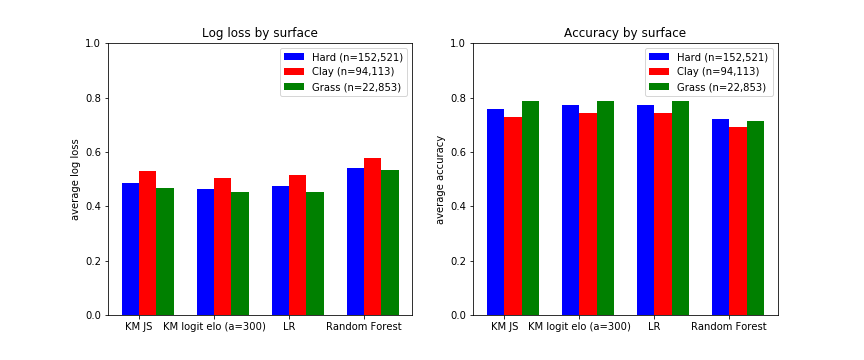
\includegraphics[scale=.6]{surface_performance3}

%Zoom in on graphs (?)
%Is this due to sample size? Probability of going three sets is higher?

By surface, models predicted grass court matches most effectively and clay court matches least effectively. As one can observe from historical tournament averages $f_t$ across surfaces, grass courts tend to yield higher serving percentages $f_{ij},f_{ji}$ than clay courts. Presumably, this is because the ball bounces more quickly off grass courts than clay courts. One explanation for observed differences is that service breaks become more likely on clay courts because $f_{ij},f_{ji}$ are lower. With service breaks more likely, it becomes harder for our models to predict the match because advantages from a current scoreline are more likely to be turned around. Hard courts, where the majority of matches took place, ultimately proved in between grass and clay in predictability. Further insight into the volatility of matches may formally shed light on differing results across surfaces.\footnote{We may calculate a measure of volatility from point-by-point sequences or a model's win probability output.}

%By nature, grass courts are faster and conducive to offensive play. Since service games are held at a higher rate, break advantages can be more decisive, which likely gave our models an edge when predicting outcomes from all scorelines. On the other hand, clay courts suit defensive play and exhibit more service breaks.  



%\subsection{Distribution of Performance}
%show a histogram of log loss scores, accuracy scores by match. Do we want this (??)



%\subsection{Variable Importance}

%Discuss relative variable importance among features in the most effective LR model. Talk about how these features relate to the point-based model or how there may be features with information the point-based model lacks (likely not, since I crafted features to represent scenarios which are embedded in the point-based model, like break point, etc). serve percentages could be analogous to beta experiments graph LR and KM together, commenting how LR jumps around more (from points and game increases, this is a matter of reactivity from correlation vs causality; lr is somewhat reacting to jumps because having a point lead is going to be more associated with winners.)

\section{Visualizing Win Probability}

As the most effective Logistic Regression and KM models were not far off in predictive performance, we now visualize their forecasts with several tour-level matches. 

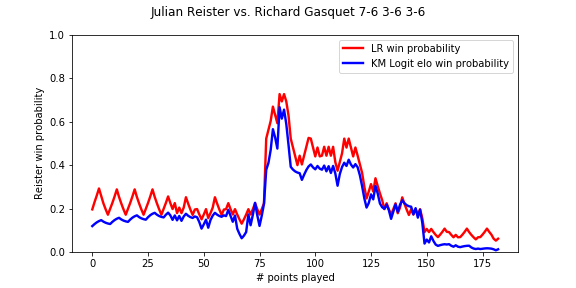
\includegraphics[scale=.7]{reister_gasquet}

Over the first thirty points of the match, the contrast between our models is reminiscent of 4.3.3. Since our Logistic Regression model has learned specific coefficients for the ``point\_diff'' feature, Reister's win probability spikes up and down noticeably as he and Gasquet exchange games on serve. Our KM logit elo model seems to have set $t = f_{ij} + f_{ji}$ to a high value, expecting frequent service holds and producing a relatively static win probability over this time frame. While we can communicate the relative importance of service breaks with constraint $t=f_{ij}+f_{ji}$, there is no direct method for controlling probability fluctuations with Logistic Regression.

Over the last thirty points of the match, consider how Reister's win probability slowly declines according to the KM model, while it remains approximately constant according to Logistic Regression. One drawback of our Logistic Regression feature sets was that they could not distinguish between situations whose score differentials are equivalent. As Gasquet maintains a break advantage through the end of third set, this explains logistic regression's behavior, since score differentials remain similar.

In general, consider a player serving at (1,1,5,4,3,0) and one serving at (1,1,1,0,3,0). In the first situation, the player serving wins the match if he wins any of the next three points. From the second scenario, the player serving holds a break advantage early in the final set, from which the returner has many more chances to come back. Assuming each player serves at $f_i=f_j=.64$, our point-based win-probability equation suggests a substantial difference between these two scenarios:

\begin{center}
$P_m(1,1,5,4,3,0) = .994$

$P_m(1,1,1,0,3,0) = .800$
\end{center}

Although the first situation is clearly favorable, Logistic Regression will observe equivalent differentials (set\_diff, game\_diff, and point\_diff) and compute approximately the same probability in both scenarios.$\footnote{\text{After fitting coefficients, P($\bold{x}$) = P($s_i-s_j,g_i - g_j,{x}_i -{x}_j)= \frac{e^{(\beta_0 + \beta_1(s_i-s_j) + \beta_2(g_i-g_j)+\beta_3(x_i-x_j)}}{1+e^{(\beta_0 + \beta_1(s_i-s_j) + \beta_2(g_i-g_j)+\beta_3(x_i-x_j)}}$}$, $\newline and P(1,0,5,4,3,0) = P(1,0,1,0,3,0) by symmetry.}$

%$\footnote{after fitting coefficients for the equation $P(win) = logit(s_i,s_j,g_i,g_j,{x}_i,{x}_j) = \frac{e^{(c_1s_i+c_2s_j+c_3g_i+c_4g_j+c_5x_i+c_6x_j}}{55}$, coefficients $ c_1 \approx c_2, c_3 \approx c_4,c_5 \approx c_6$ by symmetry and therefore}$

%In general, a player serving at (1,1,5,4,3,0) will have approximately the same win probability as one serving at (1,1,1,0,3,0). However, in the first situation, the player serving wins the match if he wins any of the next three points. From the second scenario, the player serving only holds a break advantage early in the set, from which the returner has many more chances to come back. Assuming each player serves at $f_i=f_j=.64$, our win-probability equation suggests a substantial difference between these two scenarios:

In a similar example, Logistic Regression may also fail to notice when a higher-ranked player is about to lose a close match.

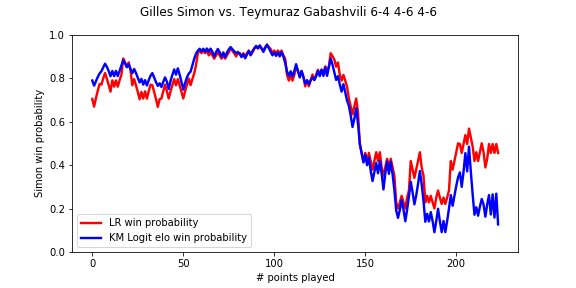
\includegraphics[scale=.7]{simon_gabashvili}

Simon leads for most of the match until Gabashvili comes back to force the third set. At the end of the third set, Gabashvili serves out the match from 5-4, yet the model fails to detect that Simon is about to lose. This is because, with sets at 1-1 and game differentials nearly even, Simon's Elo advantage outweighs his current scoreline disadvantage. Consequentially, his win-probability hovers between 50\% as he loses the match, rather than fall toward 0. While we considered several score-based interaction terms to prevent scenarios like this, adding them to our feature set did not significantly change results. Still, when comparing model performance in specific scenarios, it is important to note that the KM model was specifically designed for tennis prediction while our Logistic Regression model was simply fed score-related features that seemed helpful. Despite apparent faults, observed performance suggests potential in further exploring machine learning methods.



\chapter{Conclusion}

For the first time, we have documented the performance of in-match prediction methods on thousands of matches. While previous work only referenced individual matches or the 1992-1995 Wimbledon match dataset \citep{Klaassen2003}, we have applied methods to thousands of matches from recent years. Results from this project and Jeff Sackmann's point-by-point dataset should serve as an appropriate benchmark for future work in this field.

%future work regarding in-match prediction, we have established a benchmark and dataset against which to test prediction methods.

Although many papers have referenced Klaassen and Magnus' point-based model, none has explicitly outlined a way to correct for uncertainty stemming from small sample sizes in players' serve/return history. Applying a normalization method, such as the James-Stein estimator in 3.5, significantly boosts the performance of point-based models. By factoring in the overall ability of a player's opponents in the past twelve months, calculating $f_{ij},f_{ji}$ from the opponent-adjusted method in 3.6 offers additional predictive power. Still, none of these variations produce pre-match forecasts as effectively as Elo ratings. Using our approximation algorithm in 4.3.2, we can derive serve probabilities from any pre-match forecast $\pi_{ij}$ and historical serve parameter $t = f_{ij} + f_{ji}$. A combination of this method, using $\pi_{ij}$ derived from an Elo-based logistic regression, and our KM model ultimately produced the most reliable in-match prediction model.

Still, logistic regression's performance with a score-based feature set proved noteworthy. Machine-learning models offer potential in their ability to learn from a training set. While serve parameters $f_{ij},f_{ji}$ may be obtained from a machine-learning model's forecast, $\pi_{ij}$, our traditional point-based hierarchical Markov Model offers no comparable method to ``train'' itself from a dataset. Future work with point-based models that offers some aspect of optimization with respect to a training set may be of much interest to fans and bettors alike. For the time being, however, we have outlined several approaches to produce well-calibrated win probability forecasts at any point in a tennis match.

\section{Applications to Betting Markets}

Methods explored in this project may be applied to betting markets in several ways. First, we can take any pre-match forecast $\pi_{ij}$, derived from implied market odds, with historical serve parameter $t = f_{ij} + f_{ji}$  and produce corresponding serve probabilities $f_{ij},f_{ji}$ from method 4.3.2. As Kovalchik found that the Bookmaker Consensus Model outperformed Elo ratings \citep{Kovalchik2016}, we could likely further improve in-match prediction models by using pre-match betting odds. Next, we may back test any of our in-match prediction techniques against historical in-match odds. Betfair, an online gambling company, offers historical market data which is time-stamped yet lacks corresponding match scores. While mapping time-stamped market odds to corresponding scorelines across our point-by-point dataset proved out of scope, analyses with in-match betting data do exist. Huang demonstrated score inference from betting odds \citep{Huang2011}, and market-implied odds may serve as a benchmark against which to compare models. Finally, one may also test betting strategies with any of these models in real time, provided with up-to-date Elo ratings and $f_{ij},f_{ji}$.


%This project was intended to lay a foundation for in-match prediction. By testing models on 

\section{Future Steps}

Aside from beta experiments, all point-based models in this paper operated under the assumption that points played by each server are i.i.d. While Klaassen and Magnus concluded that deviations from i.i.d. are small enough for such models to provide a reasonable approximation \citep{KlaassenandMagnus2001}, the truth is that points within a match are not independent. Although players train themselves to ignore the score board, no player is truly capable of maintaining a constant level of play throughout every match. As soon as a player's level fluctuates, sequential points become dependent, suggesting dips or spikes in form throughout the match. Future work exploring momentum through dependencies between points, games, and sets could add another dimension of prediction to our point-based models. To start, one could quantify how much winning a point on serve affects the probability of winning the next point on serve. In total, Jeff Sackmann's point-by-point dataset offers over 100,000 matches over which to explore effects of momentum.\footnote{While we examined ATP tour-level matches, there are also corresponding WTA matches and satellite-level events for each tour.}

%Tracking a player's momentum at any point in the match, and updating serve probabilities accordingly, may also allow us to improve our models.

Explored methods in this paper were tested exclusively on ATP matches. All methods and analyses conducted in this paper may also be applied to women's WTA matches in Sackmann's point-by-point dataset and contrasted to illustrate match predictability across men's and women's tours.

\section{Visualizing Grand Slam Matches}

Below, we view win-probability graphs for several historical matches. Probabilities were generated by KM logit-elo (a=300).

\subsection{\mbox{Roger Federer vs. Rafael Nadal Australian Open 2017 Final}}

Earlier this year, Roger Federer overcame Rafael Nadal in the Australian Open final 6-4 3-6 6-1 3-6 6-3.

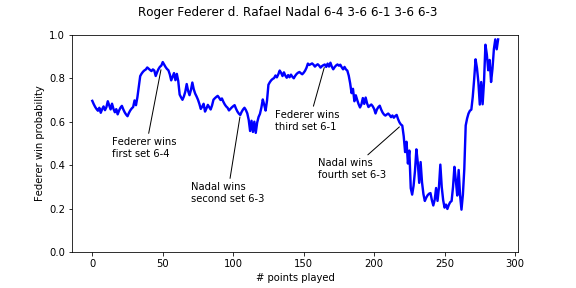
\includegraphics[scale=.7]{federer_nadal_ao_17}

\subsection{\mbox{Stanislas Wawrinka vs. Novak Djokovic French Open 2015 Final}}

With Djokovic facing pressure complete a career Grand Slam with a French Open title for years,\footnote{This entails winning each of the grand slams once: Australian Open, French Open, Wimbledon, US Open.} the title finally appeared within his grasp as he knocked out Nadal, then a 9-time French Open champion, en route to the 2015 final. However, Wawrinka had other plans on this day, turning around the match and overpowering Djokovic with unwavering determination.

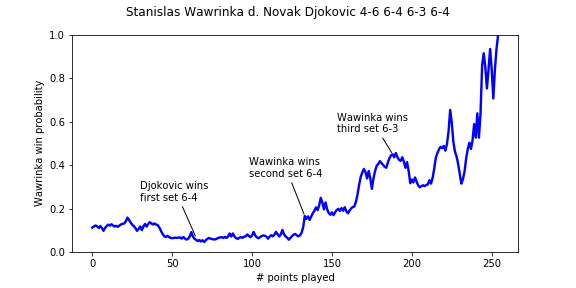
\includegraphics[scale=.7]{wawrinka_djokovic_fo_15}

\subsection{Novak Djokovic vs. Roger Federer US Open 2011 Semi-Final}

In one of the most famous comebacks in tennis history, Djokovic recovered from a two-set deficit before escaping defeat at 3-5 15-40 on Federer's serve in the final set.\footnote{If one were to consider Djokovic's decision to hit an all-or-nothing return winner at 3-5 15-40 in the fifth set, we could have computed his win probability to be even less than $p=.015$, as Federer would have surmised (\url{https://www.theguardian.com/sport/2011/sep/11/us-open-2011-federer-djokovic}). Calculating in-match win probability within points based on shot-selection is realistic nowadays, thanks to Jeff Sackmann's match charting project and recent data analyses with Hawkeye ball-tracking data.}

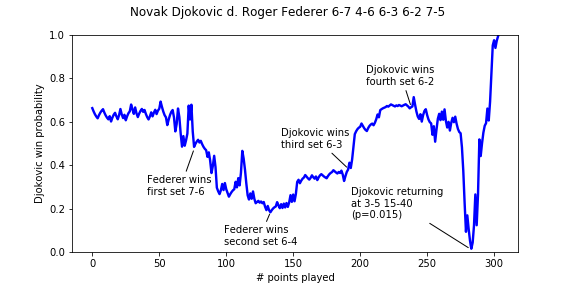
\includegraphics[scale=.7]{djokovic_federer_uso_11}




\bibliography{references}

\end{document}